\setchapterpreamble[u]{\margintoc}
\chapter{Հավանականություն}
\labch{probability}

\emergencystretch 2em

\section{Պատահական փորձ}

Հաճախ կյանքում հանդիպում ենք այնպիսի իրավիճակների, երբ այս կամ այն գործողության/երևույթի արդյունքը հնարավոր չէ գուշակել, ասենք՝
\begin{itemize}
    \item ի՞նչ թիվ կընկնի, եթե նետենք զառը
    \item ո՞ր կողմի վրա կընկնի նետված մետաղադրամը
    \item ո՞վ կհաղթի, եթե շախմատ խաղաք Լևոն Արոնյանի հետ
    \item եթե դուրս գանք փողոց ու կանգնեցնենք պատահական անցորդի, ի՞նչ կլինի նրա անունը
    \item եթե դուրս գանք փողոց ու կանգնեցնենք պատահական անցորդի, որքա՞ն կլինի նրա հասակը
    \item քանի՞ րոպեից կժամանի $62$ համարի ավտոբուսը
\end{itemize}
և այլն։ Իրոք, մինչև զառը չնետենք, կանգառում չսպասենք, խաղը չխաղանք՝ չենք կարող ասել հստակ արդյունքը։ 
Չնայած դրան՝ կարող ենք այնուամենայնիվ ինչ-որ ենթադրություններ անել հնարավոր արդյունքի մասին, այսինքն՝ համեմատել, թե հնարավոր ելքերից որը ավելի մեծ շանս ունի  տեղի ունենալու, որը՝ ավելի փոքր։ 

Այլ կերպ ասած՝ թեև հնարավոր չէ հստակ գուշակել արդյունքը, բայց կարելի է խոսել հնարավոր ելքերի \textit{հավանականությունների} մասին։ Օրինակ՝
\begin{itemize}
    \item \textit{զառ նետելիս}  

    \begin{itemize}
        \item[-] հնարավոր է վեց տարբերակ՝\marginnote{տարբերակներից յուրաքանչյուրը կան\-վա\-նենք \textit{տարրական ելք} կամ պար\-զա\-պես՝ \textit{ելք}} $1$, $2$, $3$, $4$, $5$ կամ $6$
        
        \item[-] քանի որ դրանցից ոչ մեկը մյուսի նկատմամբ առավելություն չունի, ապա բոլոր ելքերն ունեն նույն հավանականությունը
    \end{itemize}

    \item \textit{մետաղադրամ նետելիս} 

    \begin{itemize}
        \item[-] կա երկու ելք՝ գիր կամ ղուշ
        
        \item[-] եթե մետաղադրամը իսկական է, երկու ելքերի դուրս գալու հավանականությունը նույնն է՝ $50\%$-ով գիր, $50\%$-ով՝ ղուշ

        \item[-] հնարավոր է, որ մետաղադրամը կեղծված լինի այնպես, որ այն ավելի հակված լինի ասենք՝ ընկնելու գիր․ այդ դեպքում գիր ընկնելու հավանականությունն ավելի մեծ կլինի, քան ղուշ ընկնելունը
    \end{itemize}

    \item \textit{շախմատ խաղալիս}

    \begin{itemize}
        \item[-] կա երկու ելք՝ հաղթում եք կամ Դուք, կամ Լևոն Արոնյանը
        \item[-] գրեթե $100\%$-անոց հավանականությամբ հաղթողը կլինի Արոնյանը
    \end{itemize}
    
    \item \textit{պատահական մարդու անունը հարցնելիս}

    \begin{itemize}
        \item[-] կան հարյուր հազարավոր հնարավոր ելքեր
        \item[-] դրանցից որոշները (ասենք՝ Անի կամ Դավիթ) ավելի հավանական են, քան մյուսները
        \item[-] միջինում $1000$ անցորդից մոտ $20$-ի անունը կլինի Անահիտ, ևս $17$-ինը՝ Արմեն, և այլն
    \end{itemize}
        
    \item \textit{պատահական մարդու հասակը հարցնելիս}

    \begin{itemize}
        \item[-] կան անվերջ թվով ելքեր․ մարդու հասակը կարող է լինել, ասենք, \marginnote{նկատի ունենք ճշգրիտ հասակը (նանո\-մետ\-րերի ճշտությամբ), ոչ կլորացված} $(60, 240)$ սմ միջակայքից ցանկացած թիվ 
        \item[-] ավելի հավանական է, որ հասակները լինեն $(160, 180)$ միջակայքում, քան ասենք՝ $(210, 230)$
    \end{itemize}

    \item \textit{$62$ համարի ավտոբուսին սպասելիս}

    \begin{itemize}
        \item[-] այս հարցին հավանականությունների տեսությունն անզոր է պատասխանել
    \end{itemize}
\end{itemize}
\question{Ի՞նչ եք կարծում, որքա՞ն է հավանականությունը, որ պատա\-հական վերցված մարդու հասակը լինի $174.12345678912345...$ սմ։} 
Յուրաքանչյուր այսպիսի երևույթ կանվանենք \textit{պատահական փորձ} ($=$ բան, որի ելքը/արդյունքը չգիտենք)։ Ամեն մի պատահական փորձի համար նրա բոլոր հնարավոր ելքերը կհավաքենք մեկ բազմության մեջ և կանվանենք այն \textit{բոլոր ելքերի բազմություն} կամ \marginnote{անգլերեն՝ {\it sample space}} \textit{նմուշային տարածություն} (կնշանակենք $\Omega$ տառով)․
\[
\Omega = \{ \text{տվյալ պատահական փորձի բոլոր հնարավոր ելքերը} \}
\]

\begin{example}
Մետաղադրամ նետելը պատահական փորձ է, որի ելքերն են՝\marginnote{անգլերեն՝ {\it heads} և {\it tails}}
\[
\Omega = \{\text{գիր}, \text{ղուշ}\} = \{\text{Գ}, \text{Ղ}\} = \{{\rm H}, {\rm T}\}  
\]
\end{example}

\begin{example}
Ցանկացած ֆուտբոլային խաղ պատահական փորձ է, որի ելքը խաղի հաշիվն է․ քանի դեռ խաղը տեղի չի ունեցել, հաշիվը չգիտենք։ Եթե պայմանավորվենք օրինակ՝
\[
\text{Փյունիկ } 2 - 1 \text{ Ալաշկերտ}
\]
ելքը նշանակել $(2, 1)$-ով, բոլոր ելքերը կլինեն՝
\[
\Omega = \{(0,0),\ (0,1),\ (1,0),\ (1,1),\ (2,0),\ \dots \}
\]
\end{example}

\begin{example}
Եթե պատահական ինչ-որ պահի դուրս գաք կանգառ և սպասեք, թե քանի րոպեից կգա ավտոբուսը, դա նույնպես կլինի պատահական փորձ։ 

Եթե համարենք, որ ավտոբուսներն անցնում են ժամը մեկ, հնարավոր է, որ հաջորդ ավտոբուսը գա $45$ րոպե անց, հնարավոր է՝ կես ժամ կամ $29.5$ րոպե անց, կամ միգուցե՝ $\pi$ րոպե անց․
\[
\Omega = (0, 60)
\]
Նորից, պայմանավորվենք ավտոբուսի գալու ժամանակը չկլորացնել րոպեի ճշտությամբ\marginnote{այսինքն՝ $\pi$ րոպե $\ne 3$ կամ $3.14$ րոպե}։ Բայց այդ դեպքում $(0, 60)$ միջակայքում կան անվերջ քանակով թվեր, որոնցից ոչ մեկը մյուսների նկատմամբ առավելություն չունի։ Իրոք, ինչո՞ւ պիտի ավտոբուսի $35.1908470$ րոպե հետո գալու հավանականությունը ավելի փոքր կամ ավելի մեծ լինի, քան ասենք $35.1908480$ կամ $35.1908471$ րոպե հետո գալունը։ 

Ստացվում է, որ $(0, 60)$ միջակայքում կան անվերջ քանակով թվեր, և յուրաքանչյուրի տեղի ունենալու հավանականությունը նույնն է, ինչ մյուսներինը։ Ուրեմն (որքան էլ ոչ ինտուիտիվ թվա) ելքերից ցանկացածի հավանականությունը․․․ $0$ է։ 

Սա \textbf{չի նշանակում,} որ ոչ մի ելք հնարավոր չէ, և ավտոբուսը երբեք էլ չի գալու․ \marginnote{\href{https://www.youtu.be/ZA4JkHKZM50}{այս մասին ավելի համոզիչ}}\textit{հավանականությունը $0$ լինել} $\ne$ \textit{հնարավոր չլինել։} Պարզապես նստել ու սպասել, որ ավտոբուսը կգա հենց ուղիղ $35.1908480$ րոպե անց, և ոչ մի վայրկյան, միլիվայրկյան ու նանովայրկյան ուշ կամ շուտ, նման բանի տեղի ունենալու շանսերը զրոյական են։
\end{example}

Նկատենք, որ կախված փորձից՝ ելքերի բազմությունը կարող է տարբեր քանակությամբ տարրեր ունենալ․ առաջին օրինակում $\Omega$-ն երկու ելքից էր բաղկացած, երկրորդում (ըստ էության) ու երրորդում՝ անվերջ թվով ելքերից։ Ընդ որում եթե երրորդ օրինակում $\Omega$-ն միջակայք էր, ապա երկրորդում $\Omega$-ն բնական թվերի զույգերից բաղկացած բազմություն էր։ 

Նշենք, որ եթե բազմության տարրերը կարելի է բնական թվերով համարակալել (այսինքն՝ $1$-ին տարր, $2$-րդ տարր, $\dots$), ապա այն անվանում ենք \textit{հաշվելի,} իսկ եթե բազմությունը միջակայք է, ապա այն \href{https://www.youtu.be/nU3fzO94lBw}{չենք կարող} համարակալել և անվանում ենք \textit{անհաշվելի։} Սա է պատճառը, որ նման միջակայքերի դեպքում ունենք շատ-շատ մեծ քանակությամբ անվերջ հատ ելքեր, որոնցից յուրաքանչյուրի հավա\-նականությունը $0$ է, թեև դրանք բոլորն էլ հնարավոր ելքեր են։

% \question{}


\section{Պատահույթներ}

Եկեք այժմ ներմուծենք հավանականությունը հաշվելու համար ան\-հրա\-ժեշտ որոշակի գործիքներ։ 

Ենթադրենք նետում ենք զառ․
\[
\Omega=\{1,\, 2,\, 3,\, 4,\, 5,\, 6\}
\]
Կարող ենք, օրինակ, հարցնել՝ արդյո՞ք զառը կընկնի
\begin{itemize}
    \item $3$
    \item $1$ կամ $6$
    \item $4$-ից փոքր թիվ
    \item զույգ թիվ
    \item պարզ թիվ\marginnote{$2$, $3$, $5$ պարզ են, $4$ ու $6$-ը՝ բաղադրյալ, $1$-ը՝ ոչ պարզ, ոչ բաղադրյալ}
    \item բնական թիվ
    \item մի որևէ թիվ
    \item ոչ մի թիվ էլ չի ընկնի
\end{itemize}

\question{Ինչպե՞ս կպատասխանեիք վերջին երեք հարցերին։}

Յուրաքանչյուր դեպքում որոնվող հավանականությունը կնշանակենք $\PP$ տառով, ասենք՝
\[
\PP[\text{$1$ կամ $6$}] =\ ?
\]
կամ
\[
\PP[\text{պարզ թիվ}] =\ ?
\]

Որպեսզի էլ ավելի պարզեցնենք գրելաձևը, պայմանավորվենք բառերով «$1$ կամ $6$», «պարզ թիվ», և այլն գրելու փոխարեն ներկայացնել նշված պայմանին բավարարող թվերը \textit{բազմության} միջոցով, այսինքն՝
\[
\PP[\text{$1$ կամ $6$}]\text{-ի փոխարեն՝} \qquad 
\PP[\{1,\ 6\}]
\]
և
\[
\PP[\text{պարզ թիվ}]\text{-ի փոխարեն՝} \qquad 
\PP[\{2,\ 3,\ 5\}]
\]
քանի որ այսպես ավելի հարմար է։ Ցանկության դեպքում կարող ենք նաև այս բազմությունները նշանակել տառերով՝ $A=\{1, 6\}$ և $B=\{2, 3, 5\}$, ու պարզապես գրել՝ $\PP[A]$ և $\PP[B]$։

\question{Ո՞ր բազմությունով կներկայացնեք զույգ լինելու հարցը։ \linebreak Իսկ $3$ լինելո՞ւնը։}

Բոլոր այսպիսի հարց-բազմությունները կանվանենք \textit{պատահույթներ}\marginnote{անգլերեն՝ {\it event}}։ Փաստորեն դրանք տարրական ելքերից բաղկացած բազմություններ են, որոնց հավանականությունը փորձում ենք չափել․ եթե մեր դեպքում՝ $B=\{2, 3, 5\}$, ապա 
\[
\PP[\{2,\ 3,\ 5\}] \quad = \quad \text{հավանականությունը, որ ելքը $2$ կամ $3$ կամ $5$ է}
\]
այսինքն՝ որ ելքը $B$ բազմության տարրերից որևէ մեկն է։ Ելքի՝ զույգ թիվ լինելու պատահույթն էլ, օրինակ, կլինի $C=\{2, 4, 6\}$ բազմությունը։

\question{Ի՞նչ ցույց կտա $B \cap C$ պատահույթը։ Իսկ $A \cap B$՞-ն։}

Իրոք, ի՞նչ կլինի, եթե հատենք $B$ և $C$ բազմությունները․ կունենանք $B \cap C = \{2\}$, այսինքն՝ այն միակ ելքը, որը և՛ պարզ է ($B$ բազմությունից է), և՛ զույգ ($C$ բազմությունից է)․
\[
\PP[B \cap C] = \PP[\text{ելքը և՛ $B$-ից է, և՛ $C$-ից}]
\]
կամ այլ ձևով ասած՝ $B$-ի ու $C$-ի հատումը այդ երկուսի \textit{միաժամանակ} տեղի ունենալու պատահույթն է։

% \question{Ո՞րն է $A$ և $B$ պատահույթների հատումը։}

Նկատենք, որ երբեմն երկու պատահույթներ կարող են հատում չունենալ, օրինակ՝ $A$-ն ու $B$-ն, քանի որ չկա այնպիսի ելք, որը լինի և՛ պարզ, և՛ $\{1, 6\}$ բազմությունից։ Այդ դեպքում նրանց հատումը կլինի դատարկ բազմություն (որը նշանակում ենք $\varnothing$-ով), \marginnote{և իհարկե, եթե $A\cap B=\varnothing$, ապա դրանք միաժամանակ չեն կարող տեղի ունենալ՝ \[\PP[A \cap B] = 0\]} և կասենք, որ $A$ ու $B$ պատահույթներն \textit{անհամատեղելի} են կամ \textit{չհատվող}։

Նույն կերպ $B$-ի ու $C$-ի միավորումը՝ $B \cup C = \{2,\, 3,\, 4,\, 5,\, 6\}$ այն պատահույթն է, որ զառի թիվը կլինի պարզ կամ զույգ (կամ էլ երկուսը միաժամանակ)․
\[
\PP[B \cup C] = \PP[\text{ելքը կա՛մ $B$-ից է, կա՛մ $C$-ից}]
\]
կամ այլ ձևով ասած՝ $B$-ի ու $C$-ի հատումը այդ երկուսից \textit{գոնե մեկի} տեղի ունենալու պատահույթն է։

\begin{marginfigure}
    \centering
    \caption*{հարմար է պատահույթները ներ\-կա\-յաց\-նել այսպիսի շրջաններով}
    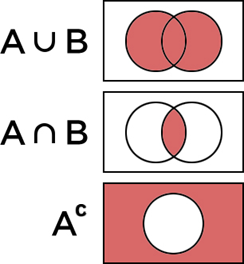
\includegraphics[width=0.75\linewidth]{chapters/chapter 8/set operations.png}
\end{marginfigure}

\warning{$B \cup C$-ում ներառված են նաև այն ելքերը, որոնք միաժամանակ երկուսին էլ պատկանում են։}

Վերջապես, եթե օրինակ՝ $B$-ն այն պատահույթն է, որ զառի ելքը պարզ է, ապա $B^c$-ով կնշանակենք դրա հակառակ պատահույթը, այսինքն՝ որ զառի ելքը պարզ \textit{չէ․}
\[
\PP[B^c] = \PP[\text{ելքը $B$-ից չէ}]
\]
Այս $B^c$ պատահույթը կանվանենք $B$ պատահույթի \textit{լրացում։} 

Նկատենք, որ ցանկացած $A$ պատահույթն ու իր $A^c$ լրացումը անհամա\-տե\-ղելի են՝ $A \cap A^c = \varnothing$, այսինքն՝ չի կարող ելքը և՛ պատկանել $A$-ին, և՛ չպատկանել $A$-ին (ասենք՝ և՛ զույգ լինել, և՛ զույգ չլինել)։

\question{Ի՞նչ կասեք $A \cup A^c$ պատահույթի մասին։ Ո՞ր բազմությունն է այն, և որքա՞ն պիտի լինի նրա հավանականությունը։}

Յուրաքանչյուր պատահական փորձի ժամանակ մեզ հետաքրքրող բոլոր պատահույթները կհավաքենք մեկ բազմության մեջ (որը կնշանակենք $\F$-ով) և այն \marginnote{անգլերեն՝ {\it event space}} կանվանենք \textit{պատահույթների տարածություն:} 

Նկատենք, որ այս $\F$-ի տարրերը բազմություններ են, այսինքն $\F$-ն ինքը բազմություններից բաղկացած բազմություն է:\marginnote{բոլորիս տանը կա տոպրակներով լցված տոպրակ․ $\F$-ը հենց այդ մեծ տոպրակն է} Քանի որ բոլոր հնարավոր ելքերի $\Omega$ բազմությունը նույնպես պատահույթ է, ապա $\Omega \in \F$։ 

Ընդհանուր առմամբ ինչպիսին էլ լինի մեր $\F$-ը, այն պետք է պարունակի ցանկացած պատահույթների հատումը, միավորումը և լրացումը․
\begin{enumerate}
    \item $\Omega$-ն և $\varnothing$-ը պատահույթներ են՝ $\Omega \in \F$, $\varnothing \in \F$

    \item ցանկացած $A$ պատահույթի լրացումը ևս պատահույթ է՝ $A^c \in \F$

    \item ցանկացած թվով պատահույթների հատումն ու միավորումը ևս պատահույթ է՝ 
    \begin{itemize}
        \item $A_1 \cap A_2 \in \F$
        \item $A_1 \cap A_2 \cap \dots \cap A_n \in \F$
        \item նույնիսկ անվերջ թվով՝ $\bigcap\limits_{n=1}^\infty A_n \in \F$
    \end{itemize}
    և
    \begin{itemize}
        \item $A_1 \cup A_2 \in \F$
        \item $A_1 \cup A_2 \cup \dots \cup A_n \in \F$
        \item նույնիսկ անվերջ թվով՝ $\bigcup\limits_{n=1}^\infty A_n \in \F$
    \end{itemize}
\end{enumerate}
կարճ ասած՝ հանգիստ կարող ենք ցանկացած գործողություն կատարել պատահույթների հետ, և արդյունքում ստացվածը կրկին անվանել «պատահույթ»։

\newpage

\question{Ենթադրենք $B$-ն զառի թվի պարզ, իսկ $C$-ն՝ զույգ լինելու պատահույթն է։ Կարո՞ղ եք $B$-ով ու $C$-ով արտահայտել պարզ, սակայն ոչ զույգ լինելու պատահույթը։}

Մինչև առաջ անցնելը նշենք, որ թեև միշտ կարող ենք հնարավոր ելքերից կազմված բոլոր բազմությունները համարել պատահույթներ ու անցնել առաջ,\marginnote{այդ դեպքում $\F$-ը կլինի $\Omega$-ի բոլոր ենթաբազմություններից բաղկացած գեր\-բազ\-մու\-թյունը} բայց երբեմն հարմար է լինում պաշտոնապես պատա\-հույթներ համարել միայն այն ելքերից բաղկացած բազմությունները, որոնք հետաքրքիր են տվյալ խնդրի տեսանկյունից։

\begin{example}
Պատկերացրեք՝ զառ ենք նետում, և եթե ընկնում է զույգ, ապա հաղթում ենք, եթե կենտ՝ պարտվում։ Այս դեպքում մեզ հետա\-քրքիր են հետևյալ երկու պատահույթների տեղի ունենալ-չունե\-նալը՝
\[
W = \{2, 4, 6\}, \qquad L = \{1, 3, 5\}
\]
և բացարձակապես հետաքրքիր չէ իմանալ՝ զառի վրայի թիվը պա՞րզ է, բաղադրյա՞լ է, $4$-ից մե՞ծ է, թե՞ $3$-ից փոքր։

Ուրեմն կարող ենք «անպետք տոպրակներն» աղբը նետել ու որպես պատահույթներ վերցնել միայն՝
\[ 
\F = \{ \varnothing,\ \{1,3,5\},\ \{2,4,6\},\ \Omega\} 
\]
\end{example}

\begin{example}
Իսկ եթե ասենք՝ նարդի խաղանք, և ինչ-որ պահի միակ հնարավոր թույլատրելի քայլը լինի $2$-ը, ապա նորից տարբերություն չկա՝ զառը կընկնի պարզ թիվ, թե բաղադրյալ․ կարևոր է միայն՝ $2$ կընկնի՞, թե՞ չի ընկնի։ 

Այսինքն՝ կարող ենք բավարարվել միայն $\{2\}$ պատահույթով և վերցնել՝
\[ 
\F = \{ \varnothing,\ \{2\},\ \{1,3,4,5,6\},\ \Omega\}
\]
\end{example}

Բարեբախտաբար, խնդիրներ լուծելիս պարտադիր չէ ամեն անգամ նշել, թե որն է $\F$-ը․ ավելորդ ֆորմալիզմից խուսափելու համար կարող ենք համարել, որ ելքերից կազմված ցանկացած բազմություն պատահույթ է, և լուծել խնդիրը։ Ավելի նուրբ դեպքերում, սակայն, սա կարող է հանգեցնել \href{https://www.youtu.be/wQQdpYhPTYM}{պարադոքսների}:


\section{Հավանականային չափ}

Բավական երկար ներածությունից հետո անցնենք մեր գլխավոր հերոսին՝ $\PP$-ին, որի միջոցով չափելու ենք բոլոր այն պատահույթների տեղի ունենալու հավանականությունները, որոնց մասին խոսեցինք վերևում։ Անվանենք այն \textit{հավանականային չափ։}\marginnote{անգլերեն՝ {\it probability measure}}

Ենթադրենք՝ կրկին նետում ենք զառը։ Կհամարենք, որ ամենամեծ («$100\%$-անոց») հավանականությունը $1$ է՝\marginnote[*+2]{նույն ինքը՝ $\PP[\Omega]=1$}
\[
\PP[\{1,\, 2,\, 3,\, 4,\, 5,\, 6\}] = 1
\]
և քանի որ բոլոր $6$ ելքերն ունեն միևնույն տեղի ունենալու հավանակա\-նությունը, դրանցից յուրաքանչյուրի հավանականությունը կլինի $\dfrac{1}{6}$՝
\newpage
\[
\PP[1]=\PP[2]=\dots=\PP[6]=\frac{1}{6}
\]
իսկ օրինակ զույգ թիվ ընկնելունը՝
\[
\PP[\{2,\, 4,\, 6\}] = \frac{3}{6} = \frac{1}{2}
\]

Նման դեպքերում, երբ ելքերից ոչ մեկի հավանականությունը մյուսից չի տարբերվում, ասում ենք, \marginnote{անգլերեն՝ {\it equiprobable}} որ բոլոր ելքերը \textit{հավասարահավանական} են։ Ինչպես վերևում տեսանք, հավասարահավանական դեպքում ցան\-կացած $A$ պատահույթի հավանականությունը հավասար է
\[
\PP[A] = \frac{\text{$A$-ի տարրերի թիվը}}{\text{բոլոր ելքերի թիվը}} = \frac{|A|}{|\Omega|}
\]

\begin{example}
Հիմա միաժամանակ նետենք երկու զառ։ Բոլոր տար\-բե\-րակները միասին՝ կունենանք $6\cdot 6 = 36$ հնարավոր ելք․
\[
\Omega = \{(x, y) \mid  1 \le x,\, y \le 6\}
\]
\marginnote{հերթականությունը կարևոր է․ $(3, 5)$ և $(5, 3)$ ելքերը \textbf{նույնը չեն}}Քանի որ դրանցից ցանկացածի տեղի ունենալու հավանականությունը նույնն է, ապա յուրաքանչյուր $(x, y)$ ելքի հավանականությունը կլինի՝
\[
\PP[(x, y)] = \frac{1}{36}
\]
իսկ օրինակ՝ երկուսի վրա էլ նույն թիվը լինելունը՝
\[
\PP[\{(1,1),\ (2,2),\ \dots,\ (6,6)\}] = \frac{6}{36} = \frac{1}{6}
\]
\end{example} 

Իսկ ի՞նչ եթե զառ նետելու փոխարեն դուրս գայինք փողոց, մոտենայինք պատահական մարդու ու հարցնեինք, թե վերջինս ձախլի՞կ է, թե՞ աջլիկ։ 

\question{Արդյո՞ք այս դեպքում ևս հավանականությունը կլիներ $\dfrac{1}{2}$:}

Քանի որ մարդկության ընդամենը $10\%$-ն է ձախլիկ, շատ ավելի (մաս\-նա\-վորապես՝ $9$ անգամ ավելի) հավանական է, որ պատահական վերցրած մարդը կլինի աջլիկ, քան ձախլիկ։ Այսինքն՝ ձախլիկ մարդու մոտենալու հավանականությունը ոչ թե $\dfrac{1}{2}=0.5$ է, այլ մոտավորապես $\dfrac{1}{10}=0.1$:

Ուրեմն այս դեպքում ունենք երկու ելք՝
\[
\Omega = \{ \text{Ձ}, \text{Ա}\}
\]
որոնք հավասարահավանական չեն, այլ
\[
\PP[\text{Ձ}] = \frac{1}{10} = 0.1, \qquad 
\PP[\text{Ա}] = \frac{9}{10} = 0.9
\]

Ընդհանուր դեպքում, եթե պատահական փորձն ունի վերջավոր քանակով հնարավոր ելքեր (ասենք՝ $n$ հատ), ապա կարող ենք այդ ելքերը համարակալել՝
\[
\Omega = \{\omega_1, \omega_2, \dots, \omega_n\}
\]
և քանի որ այդ ելքերի հավանականությունները կարող են տարբեր լի\-նել, \marginnote{մի ելքը կարող է շատ հավանական լինել, մի ուրիշը՝ պակաս հավանական} յուրաքանչյուր $k$-րդ ելքի հավանականությունը կնշանակենք $p_k$-ով՝
\[
p_1 = \PP[\omega_1], \quad p_2 = \PP[\omega_2], \quad \dots, \quad p_n = \PP[\omega_n]
\]

Բնականաբար, բոլոր ելքերի հավանականությունները գումարելով ստանալու ենք $1$՝
\[
p_1 + p_2 + \dots + p_n = 1
\]

Փաստորեն մեր $\PP$-ն մի այնպիսի ֆունկցիա է, որը վերցնում է պատահույթն ու վերադարձնում թիվ՝\marginnote{$A$-ն կարող է բաղկացած լինել միայն մեկ ելքից՝ $A=\{\omega_k\}$}
\[
\PP[A] = A \text{ պատահույթի տեղի ունենալու հավանականությունը}  
\]
ընդ որում՝ այն, թե ինչ թիվ է $\PP$-ն վերադարձնում, կախված է խնդրից։

\question{Մոտավորապես որքա՞ն է հավանականությունը (աչքա\-չա\-փով), որ պատա\-հական վերցված մարդու անունը 
\begin{itemize}
    \item $A_1 =$ սկսվում է «Ր» տառով
    \item $A_2 =$ սկսվում է «Ի» տառով
    \item $A_3 =$ վերջանում է «Ի» տառով
\end{itemize}
Ի՞նչ կասեք $\PP[A_1 \cup A_2]$-ի մասին։ Իսկ $\PP[A_1 \cup A_3]$-ի՞։}

Փորձենք պատասխանել այս հարցերին։ Նախ մոտավորապես գնահա\-տենք յուրաքանչյուր պատահույթի հավանականությունը․
\[
\PP[A_1] = 0.001, \qquad \PP[A_2] = 0.01, \qquad \PP[A_3] = 0.05
\]
Ի՞նչ է նշանակում $A_1 \cup A_2$։ Սա այն պատահույթն է, երբ տեղի ունեն $A_1$-ից ու $A_2$-ից գոնե մեկը, այսինքն՝ մարդու անունը սկսվում է կամ «Ր» տառով, կամ «Ի»։ Հետևաբար
\[
\PP[A_1 \cup A_2]
% = \PP[\text{սկսվում է «Ր»-ով կամ «Ի»-ով}]
= \PP[A_1] + \PP[A_2] = 0.06
\]
Իրոք, քանի որ մարդու անունը չի կարող միաժամանակ սկսվել այս երկու տառերով (այսինքն $A_1$-ն ու $A_2$-ը չեն հատվում), դրանց միավորման հավանականությունը հավասար կլինի դրանց առանձին-առանձին հավանականությունների գումարին։

Մյուս կողմից՝ $A_1 \cup A_3$-ը այն պատահույթն է, որ մարդու անունը սկսվում է \marginnote{քանի՞ անուն գիտեք «Ր» տառով սկսվող} «Ր»-ով \textit{և/կամ} վերջանում «Ի»-ով։ Այս անգամ արդեն $A_1$-ն ու $A_3$-ը հատվում են, անհամատեղելի չեն, նույնիսկ ավելին՝ «Ր»-ով սկսվող գրեթե ցանկացած անուն վերջանում է «Ի»-ով, և $A_1$ պատահույթի տեղի ունենալուց ինքնըստինքյան հետևում է, որ $A_3$-ը նույնպես տեղի ունի։ Ուրեմն
\[
\PP[A_1 \cup A_3] = \PP[A_3] = 0.05 \quad \textbf{այլ ոչ թե} \quad 0.051
\]
Այսպիսով երկու պատահույթների միավորման հավանականությունը \textit{ոչ միշտ} է հավասար դրանց հավանականությունների գումարին, քանի որ այդ պատահույթները կարող են հատվել (միաժամանակ երկուսն էլ տեղի ունենալ)։ Իսկ եթե դրանք անհամատեղելի են (մեկը մյուսին չեն օգնում կամ խանգարում), այդ դեպքում արդեն $\PP[A_1 \cup A_2] = \PP[A_1] + \PP[A_2]$:

Ամփոփելով մինչ այս պահը մեր պայմանավորվածությունները՝ ձևակեր\-պենք $\PP$-ի ֆորմալ սահմանումը․

\begin{definition}
Կասենք, որ $\PP$ ֆունկցիան \textbf{հավանականային չափ} է, եթե
\begin{enumerate}
    \item ցանկացած $A\in\F$ պատահույթի համար $\PP[A] \ge 0$
    
    \item $\PP[\Omega] = 1$

    \item ցանկացած\marginnote{նույնիսկ անվերջ հատ $A_n$-երի} $A_1$, $A_2$, $\dots$ չհատվող պատահույթների համար
    \[
      \PP\left[A_1 \cup A_2 \cup \dots \right] =  \PP[A_1]+ \PP[A_2]+\dots  
    \]
    այսինքն՝ $\PP\left[\bigcup\limits_{n} A_n\right] = \sum\limits_{n} \PP[A_n]$:
\end{enumerate}
\end{definition}

$\Omega$-ն, $\F$-ը և $\PP$-ն միասին կոչվում են նաև \textit{հավանականային տարա\-ծու\-թյուն} կամ \textit{եռյակ՝} $(\Omega, \F, \PP)$:


\section{Հատկություններ}

Այժմ արդեն պատրաստ ենք ծանոթանալու, թե ինչպես հաշվել տարբեր պատահույթների հավանականությունները։

\question{Որքա՞ն է անձրև գալու հավանականությունը, եթե հայտնի է, որ անձրև չգալունը $0.3$ է։}

Բնականաբար, եթե հայտնի է որևէ $A$ պատահույթի հավանականությունը, ապա կարող ենք հաշվել նաև դրա լրացման հավանականությունը․
\[
\PP[A^c] = 1 - \PP[A]
\]
Մասնավորապես, երկու անհամատեղելի պատահույթների հատման, այսինքն $\varnothing$ դատարկ պատահույթի հավանականությունը՝
\[
\PP[\varnothing] = 1 - \PP[\Omega] = 0
\]
ինչպես և պետք է լիներ։

\question{Ո՞ր հավանականությունն է ավելի մեծ՝ զառի զո՞ւյգ թիվ ընկնելունը, թե՞ $4$-ի բաժանվող թիվ ընկնելունը։}

Եթե ասենք $4$-ի բաժանվելու պատահույթը նշանակենք $A$-ով, իսկ զույգ լինելունը՝ $B$-ով․
\[
A = \{4\}, \qquad B = \{2, 4, 6\}
\]
ապա\marginnote{պատահույթները երկրաչափորեն նկա\-րե\-լիս սա անմիջապես երևում է․ եթե մի պատկերն ընկած է մյուսի մեջ, ապա այն ավելի փոքր է} $A$ բազմության ցանկացած տարր կպատկանի նաև $B$ բազմությանը, այսինքն $A$-ն կլինի $B$-ի ենթաբազմություն՝ $A \subset B$։ Հետևաբար $A$-ի հավանականությունը չի կարող մեծ լինել $B$-ինից․
\[
\text{եթե } A \subset B, \qquad \text{ապա } \PP[A] \le \PP[B]
\]

Ինչպես գիտենք, եթե պատահույթները չեն հատվում (անհամատեղելի են), ապա դրանցից որևէ մեկի տեղի ունենալու հավանականությունը հավասար է դրանց հավանականությունների գումարին։ Իսկ ի՞նչ, եթե դրանք հատվում են։

\question{Թբիլիսիում ապրողների մոտ $47\%$-ը խոսում է անգլերեն, $5\%$-ը՝ հայերեն, իսկ $2\%$-ը՝ և՛ անգլերեն, և՛ հայերեն։ Որքա՞ն է հավանականությունը, որ պատահական հանդիպած մարդու հետ կկարողանաք հաղորդակցվել։}

Քանի որ անգլերեն և հայերեն խոսողների բազմությունները հատվում են, $47\%$-ին $5\%$ գումարելու դեպքում որոշ մարդկանց (բնակչության $2\%$-ին) մեկի փոխարեն երկու անգամ կհաշվենք։ Հետևաբար պետք է գումարելուց հետո հանենք այդ $2\%$-ը, և արդյունքում կստանանք՝ $47\%+5\%-2\%=50\%$։

Այսինքն եթե ունենք որևէ երկու $A$ և $B$ պատահույթներ, դրանցից որևէ մեկի տեղի ունենալու հավանականությունը՝
\[
\PP[A \cup B] = \PP[A] + \PP[B] - \PP[A \cap B]}
\]
հավասար է առանձին հավանականությունների գումարից հանած դրանց հատման հավանականությունը։ Այս կանոնը կոչվում է \textit{կցման-արտաքս\-ման սկզբունք։}

\begin{figure}[h]
    \centering
    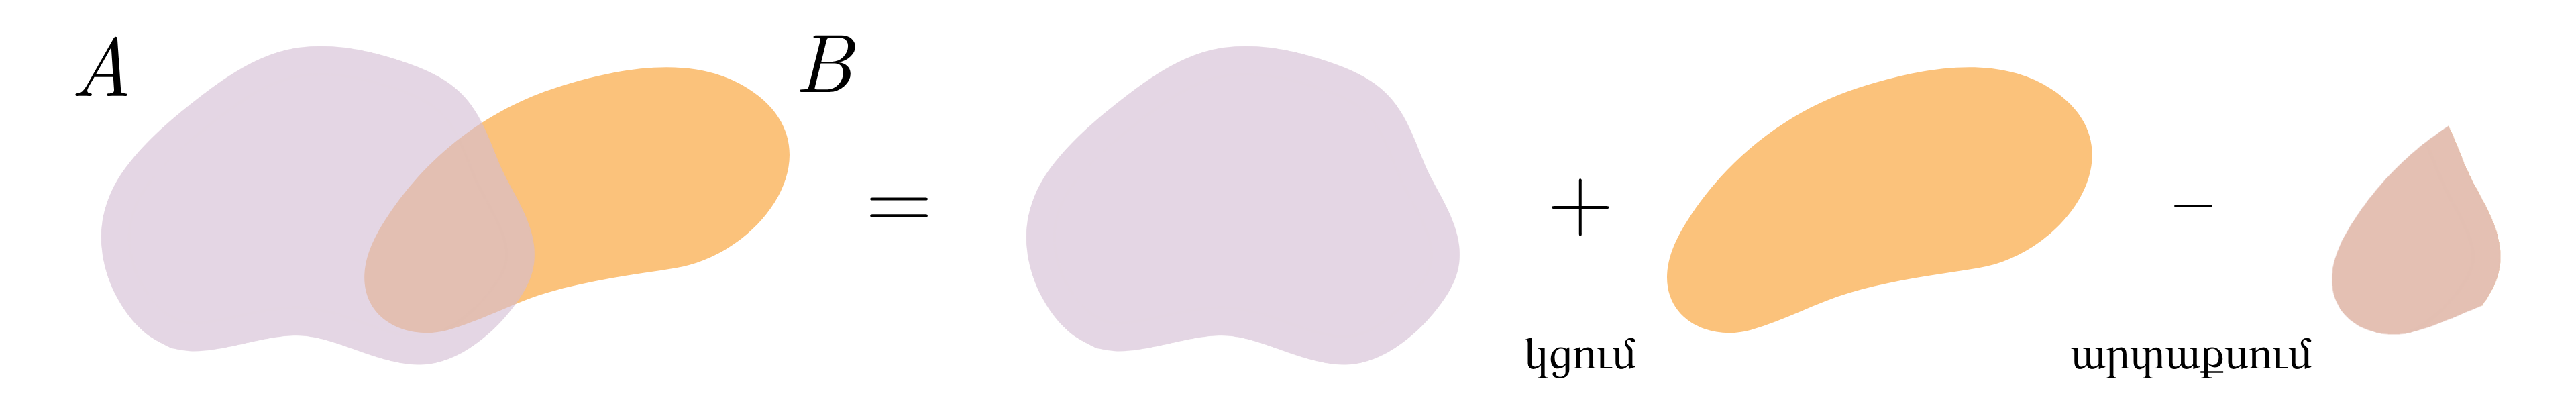
\includegraphics[width=\linewidth]{chapters/chapter 8/inclusion-exclusion.png}
\end{figure}

Մասնավորապես այս սկզբունքից հետևում է, որ 
\[
\PP[A \cup B] \le \PP[A] + \PP[B]
\]
ցանկացած $A$ և $B$ պատահույթների համար։ Ավելին, սա ճիշտ է ցանկացած թվով պատահույթների համար՝
\[
\PP\left[\bigcup_{n}A_n\right] \le \sum_n \PP[A_n]
\]
ընդ որում հավասարություն տեղի ունի միայն այն դեպքում, երբ $A_n$-երը ոչ մի ընդհանուր կետ չունեն։

\question{Կարո՞ղ եք դուրս բերել կցման-արտաքսման \href{https://www.youtube.com/shorts/xLQFOBo71w0}{սկզբունքը} երեք պատահույթների համար՝ $A$, $B$, $C$:}


\section{Պայմանական հավանականություն}

Ենթադրենք նետել ենք զառն, ու ընկել է ինչ-որ թիվ։

\newpage

\begin{description}
\item[Հարց 1․]  \textit{Որքա՞ն է հավանականությունը, որ ընկած թիվը զույգ է։}

\begin{marginfigure}
    \centering
    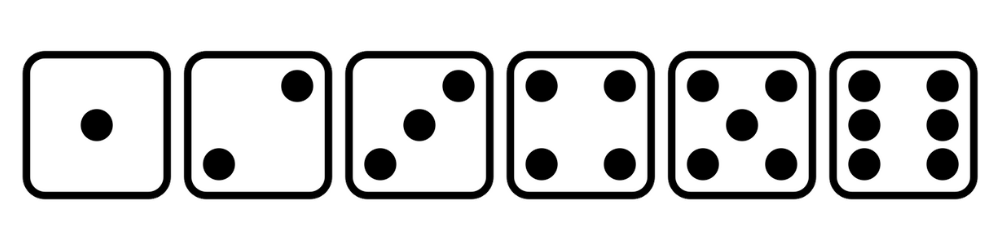
\includegraphics[width=\linewidth]{chapters/chapter 8/dice 1.png}
\end{marginfigure}

Դե քանի որ կա $6$ հնարավոր ելք, որոնցից ընդամենը $3$-ն են զույգ՝ $A = \{2, 4, 6\}$, հավանականությունը կլինի
\[
\PP[A] = \frac{3}{6} = \frac{1}{2}
\]

\item[Հարց 2․]  \textit{Որքա՞ն է հավանականությունը, որ ընկած թիվը զույգ է, եթե հայտնի է, որ այն պարզ է։}

\begin{marginfigure}
    \centering
    
\includegraphics[width=\linewidth]{chapters/chapter 8/dice 2.png}
\end{marginfigure}

Եթե ինչ-որ կերպ գիտենք, որ զառի թիվը պարզ է, նշանակում է՝ այն չի կարող լինել $1$, $4$ կամ $6$։ Հետևաբար եթե այս երեքը ջնջենք ելքերի բազմությունից, տակը կմնա \textit{երեք} հնարավոր ելք՝ $B = \{2, 3, 5\}$։ Այս երեքից միայն մեկն է զույգ, հետևաբար հավանականությունը կլինի $\dfrac{1}{3}$:
\end{description}

Այսպիսով երկրորդ դեպքում, քանի որ կողքից հավելյալ տեղեկություն ունեինք, պատասխանը փոխվեց։ Պատճառն այն է, որ զառի թվի պարզ լինելու \textit{պայմանը} նշանակում է՝ հնարավոր են միայն այն ելքերը, որոնք պատկանում են $B$ բազմությանը։ Ուրեմն այդ \textit{պայմանի ներքո} մեզ մնում են միայն $A \cap B$ բազմության մեջ եղած՝ և՛ զույգ, և՛ պարզ ելքերը։

\begin{definition}
Երկու $A$ և $B$ պատահույթների համար\marginnote{եթե $\PP[B] \ne 0$}
\[
\PP[A \mid B] = \frac{\PP[A \cap B]}{\PP[B]}
\]
թիվը կանվանենք $A$-ի (պայմանական) \textbf{հավանականություն $B$ պայմանով։}
\end{definition}

Այլ կերպ ասած՝ եթե ունենք հավելյալ տեղեկություն/պայման, որ $B$ պատահույթը տեղի ունի, ապա փոխանակ նայենք, թե բոլոր $\Omega$ ելքերից որո՞նք են $A$-ի մեջ, $\Omega$-ն շպրտում ենք, վերցնում միայն $B$-ն, և նայում, թե $B$-ի տարրերից որո՞նք են $A$-ի մեջ։ 

\begin{figure}[h]
    \centering
    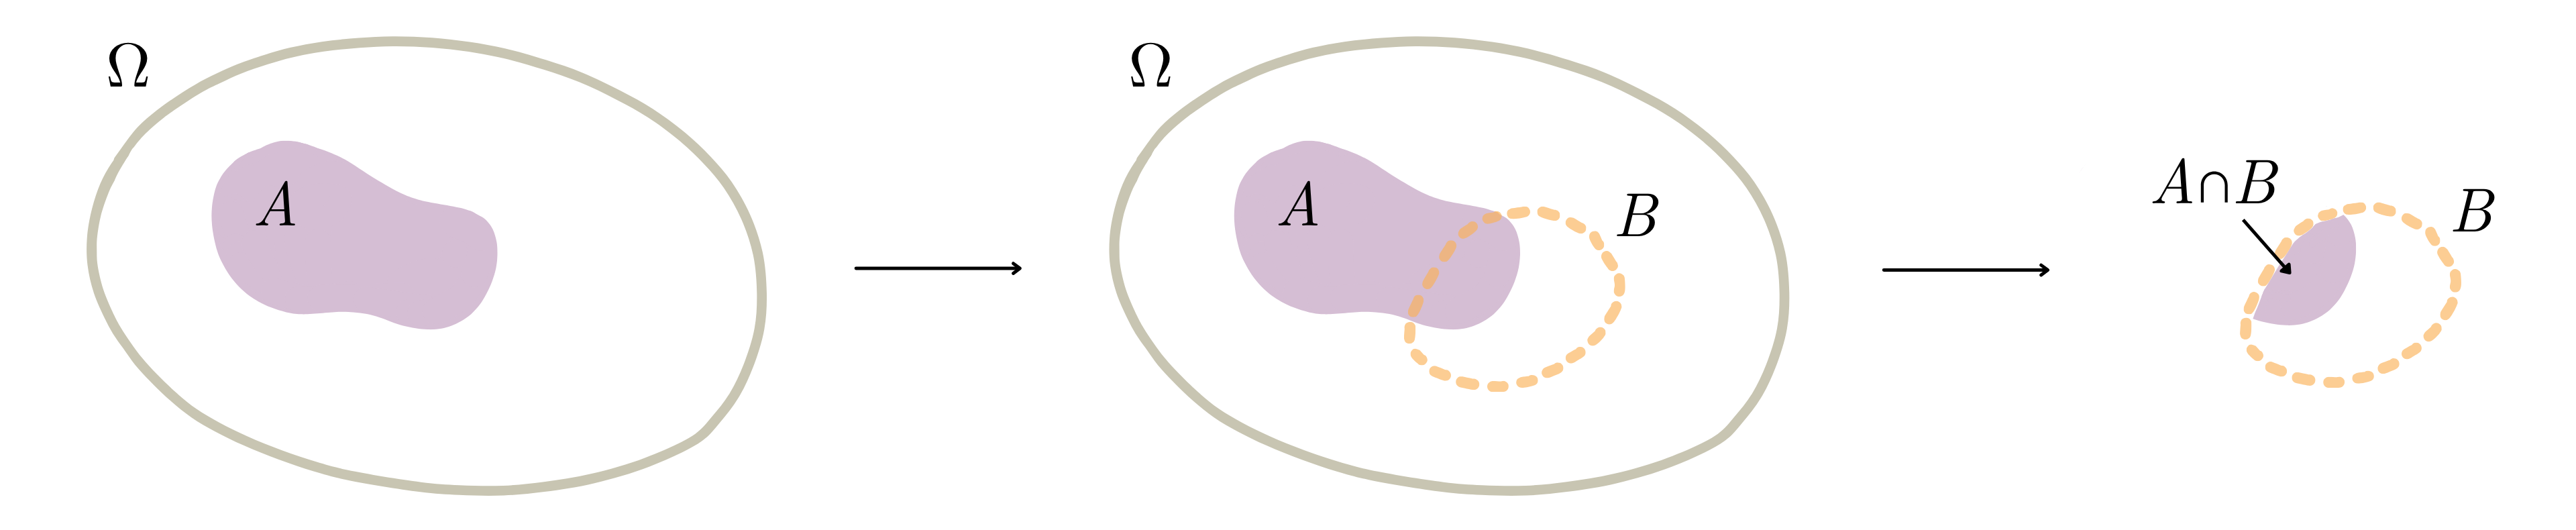
\includegraphics[width=\linewidth]{chapters/chapter 8/conditional.png}
\end{figure}

$\PP[A \mid B]$ թիվը ցույց է տալիս $A \cap B$-ի \textit{մասնաբաժինը} $B$-ի մեջ, այսինքն՝ $B$-ի որքա՞ն մասն\marginnote{քանի՞ տոկոսը} է կազմում $A$-ի հետ ունեցած հատումը։ 

Զառերի օրինակում՝
\[
\PP[\text{զույգ} \mid \text{պարզ է}]
= \PP[A \mid B]
= \frac{\PP[A \cap B]}{\PP[B]}
= \frac{\PP[\{2\}]}{\PP[\{2, 3, 5\}]}
= \frac{1/6}{3/6} = \frac{1}{3}
\]

\begin{example}
Նետել ենք երկու զառ։ Որքա՞ն է հավանականությունը, որ առաջին զառն ընկել է $2$, եթե զառերի գումարը $5$-ից մեծ չէ։

\newpage 

Առհասարակ հնարավոր է $36$ հատ ելք, որոնցից միայն $6$-ի դեպքում է առաջին զառն ընկնում $2$։ Բայց քանի որ \textit{գիտենք,} որ զառերի գումարը $5$ է, հնարավոր ելքերը լինում են ընդամենը $10$-ը․

\begin{center}
\begin{tabular}{c|*{6}{c}}
\toprule
& \dieimg{1} & \dieimg{2} & \dieimg{3} & \dieimg{4} & \dieimg{5} & \dieimg{6} \\
\midrule
\dieimg{1} & $\mathbf{2}$ & $\mathbf{3}$ & $\mathbf{4}$ & $\mathbf{5}$ & $6$ & $7$ \\
\dieimg{2} & $\mathbf{3}$ & $\mathbf{4}$ & $\mathbf{5}$ & $6$ & $7$ & $8$ \\
\dieimg{3} & $\mathbf{4}$ & $\mathbf{5}$ & $6$ & $7$ & $8$ & $9$ \\
\dieimg{4} & $\mathbf{5}$ & $6$ & $7$ & $8$ & $9$ & $10$ \\
\dieimg{5} & $6$ & $7$ & $8$ & $9$ & $10$ & $11$ \\
\dieimg{6} & $7$ & $8$ & $9$ & $10$ & $11$ & $12$ \\
\bottomrule
\end{tabular}
\end{center}

Այս $10$-ից միայն $3$-ի դեպքում է առաջին զառը ընկնում $2$, ուստի պատասխանն է $\dfrac{3}{10} = 0.3$:
\end{example}

\question{Որքա՞ն է հավանականությունը, որ Թբիլիսիում բնակվող պատա\-հական վերցված հայը խոսում է անգլերեն։}


\section{Բայեսի բանաձև}

Ենթադրենք $A$-ն ու $B$-ն զրոյից մեծ հավանականությամբ որևէ պատահույթներ են։ Եթե գիտենք $B$ պայմանի դեպքում $A$-ի տեղի ունենալու հավանականությունը, ինչպե՞ս ստանանք հակառակը՝ $A$ պայմանի դեպքում $B$-ի տեղի ունենալու հավանականությունը։

Գրենք $\PP[B \mid A]$-ի բանաձևը․
\[
\PP[B \mid A]
= \frac{\PP[B \cap A]}{\PP[A]}
= \frac{\PP[A \cap B]}{\PP[A]}
= \frac{\PP[A \mid B] \cdot \PP[B]}{\PP[A]}
\]
Հիասքանչ․ \marginnote{\href{https://upload.wikimedia.org/wikipedia/commons/c/c9/Bayes_theorem_visual_proof.svg}{պատկերավոր ապացույց}} $A$-ի ու $B$-ի տեղերը փոխվեցին։ Ստացվեց, որ ${\PP[B \mid A]}$-ն արտահայտեցինք ${\PP[A \mid B]}$-ով։ Այս արդյունքը կոչվում է \textit{Բայեսի բանաձև։}

\begin{example}
Բնության մեջ հրդեհներ տեղի են ունենում հազարից մեկ, ենթադրենք՝ $0.01$ հավանականությամբ, ընդ որում դրանցից $90\%$-ում առաջանում է տեսանելի ծուխ։ Մյուս կողմից՝ խորոված անելիս նույնպես ծուխ է առաջանում, և օրը ցերեկով ծուխ տեսնելու հավանականությունը այնքան էլ ցածր չէ, ասենք՝ $10\%$։ 

Նայում եք հեռուն և տեսնում ծուխ։ Որքա՞ն է հավանականությունը, որ Ձեր տեսածը հրդեհ է։
Նախ եթե $F$-ով նշանակենք հրդեհ, իսկ $S$-ով՝ ծուխ լինելու հավանականությունը, կունենանք՝
\[
\PP[F] = 0.01, \qquad \PP[S] = 0.1
\]
և $\PP[S \mid F] = 0.9$: Ուրեմն ըստ Բայեսի բանաձևի՝
\[
\PP[F \mid S] = \frac{\PP[S \mid F] \cdot \PP[F]}{\PP[S]} = \frac{0.01 \cdot 0.9}{0.1} = 0.09
\]
Անհանգստանալու կարիք չկա․ ամենայն հավանականությամբ ծուխը խորովածից է։
\end{example}


Քննարկենք ևս մի հետաքրքիր խնդիր։ Պատկերացրեք՝ ունենք մի համալսարան, որտեղ
\begin{itemize}
    \item կանանց $10\%$-ն է ձախլիկ
    \item տղամարդկանց $15\%$-ն է ձախլիկ
    \item ուսանողների $\dfrac{3}{5}$-ը կին են, մյուսները՝ տղամարդ
\end{itemize}

Որքա՞ն է հավանականությունը, որ պատահական վերցված ուսանողը կլինի ձախլիկ։

% \begin{figure}[h]
%     \centering
%     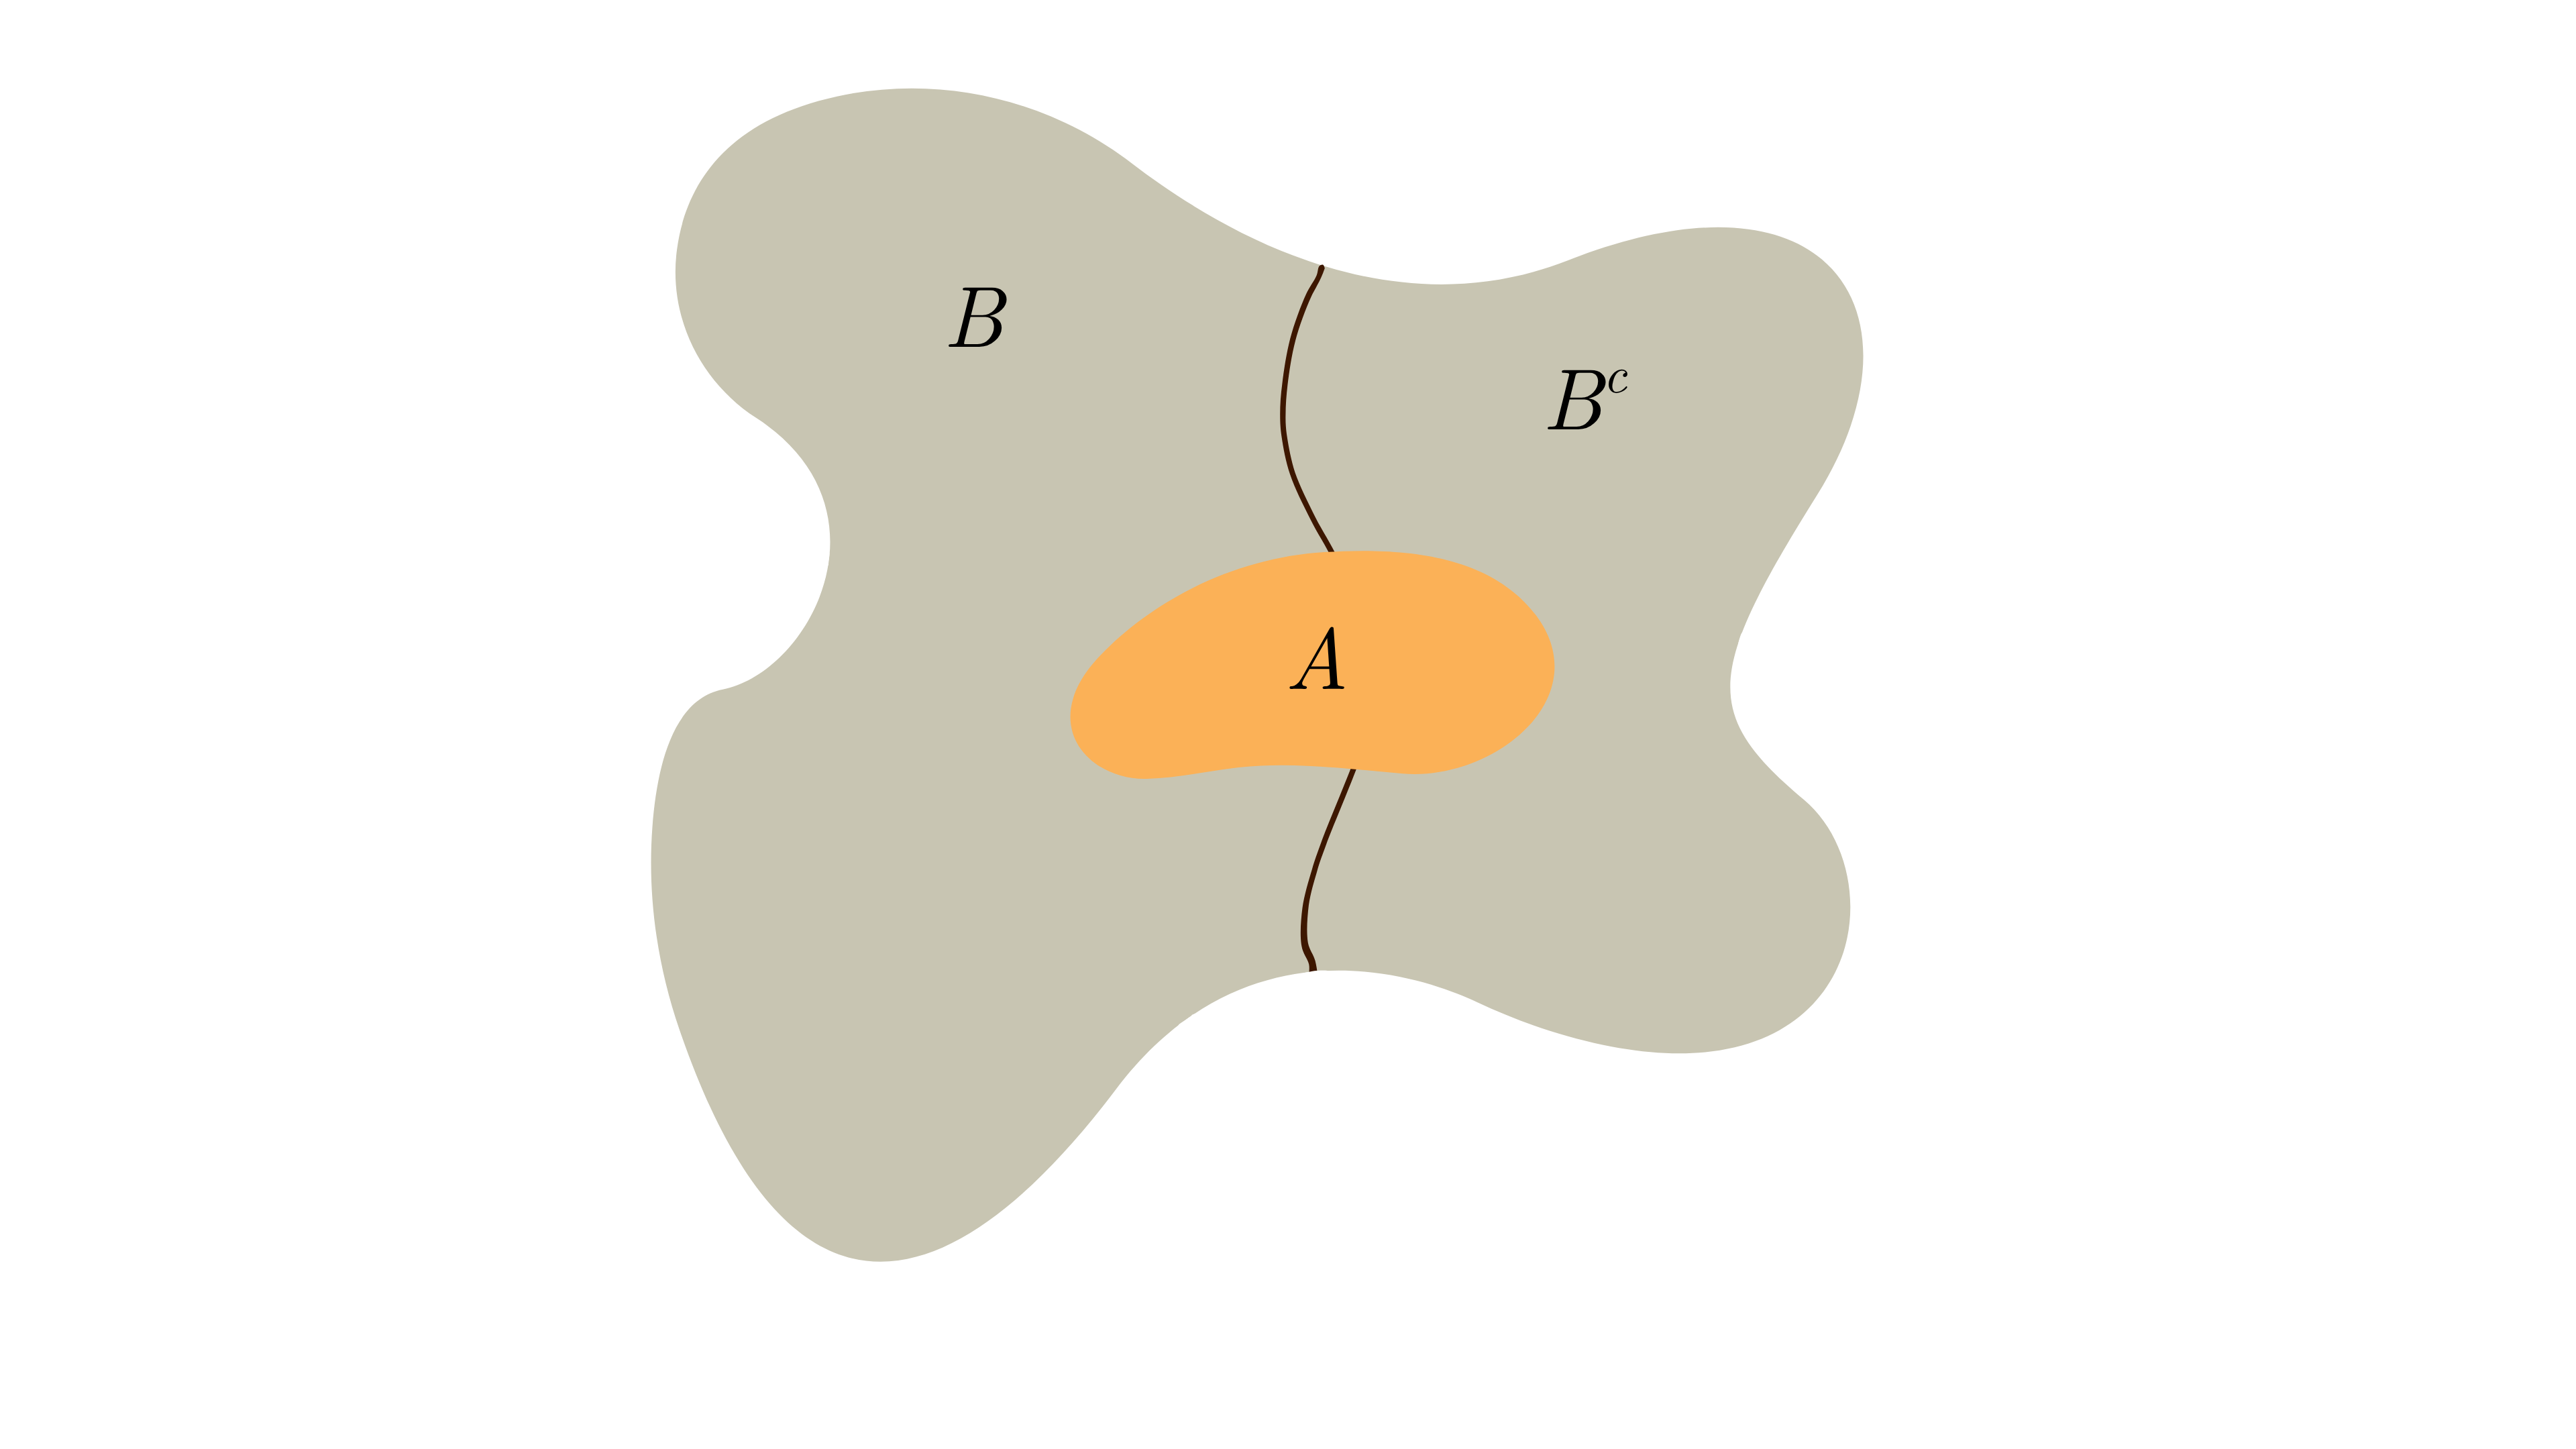
\includegraphics[width=0.7\linewidth]{chapters/chapter 8/total probability 1.png}
% \end{figure}

Նախ $A$-ով նշանակենք կին լինելու պատահույթը,\marginnote[*+1]{$B^c$-ն կլինի տղամարդ լինելունը} իսկ $B$-ով՝ ձախլիկ լինելունը։ Այդ դեպքում ձախլիկներին կարող ենք բաժանել երկու չհատվող մասերի՝
\[
\big\{\text{ձախլիկներ}\big\}
\; = \;  \big\{\text{կին ձախլիկներ}\big\} \; \cup  \; \big\{\text{տղամարդ ձախլիկներ}\big\}
\]
կամ որ նույնն է՝
\[
\PP[A] = \PP[A \cap B] + \PP[A \cap B^c]
\]
\begin{figure}[h]
    \centering
    \subfloat{{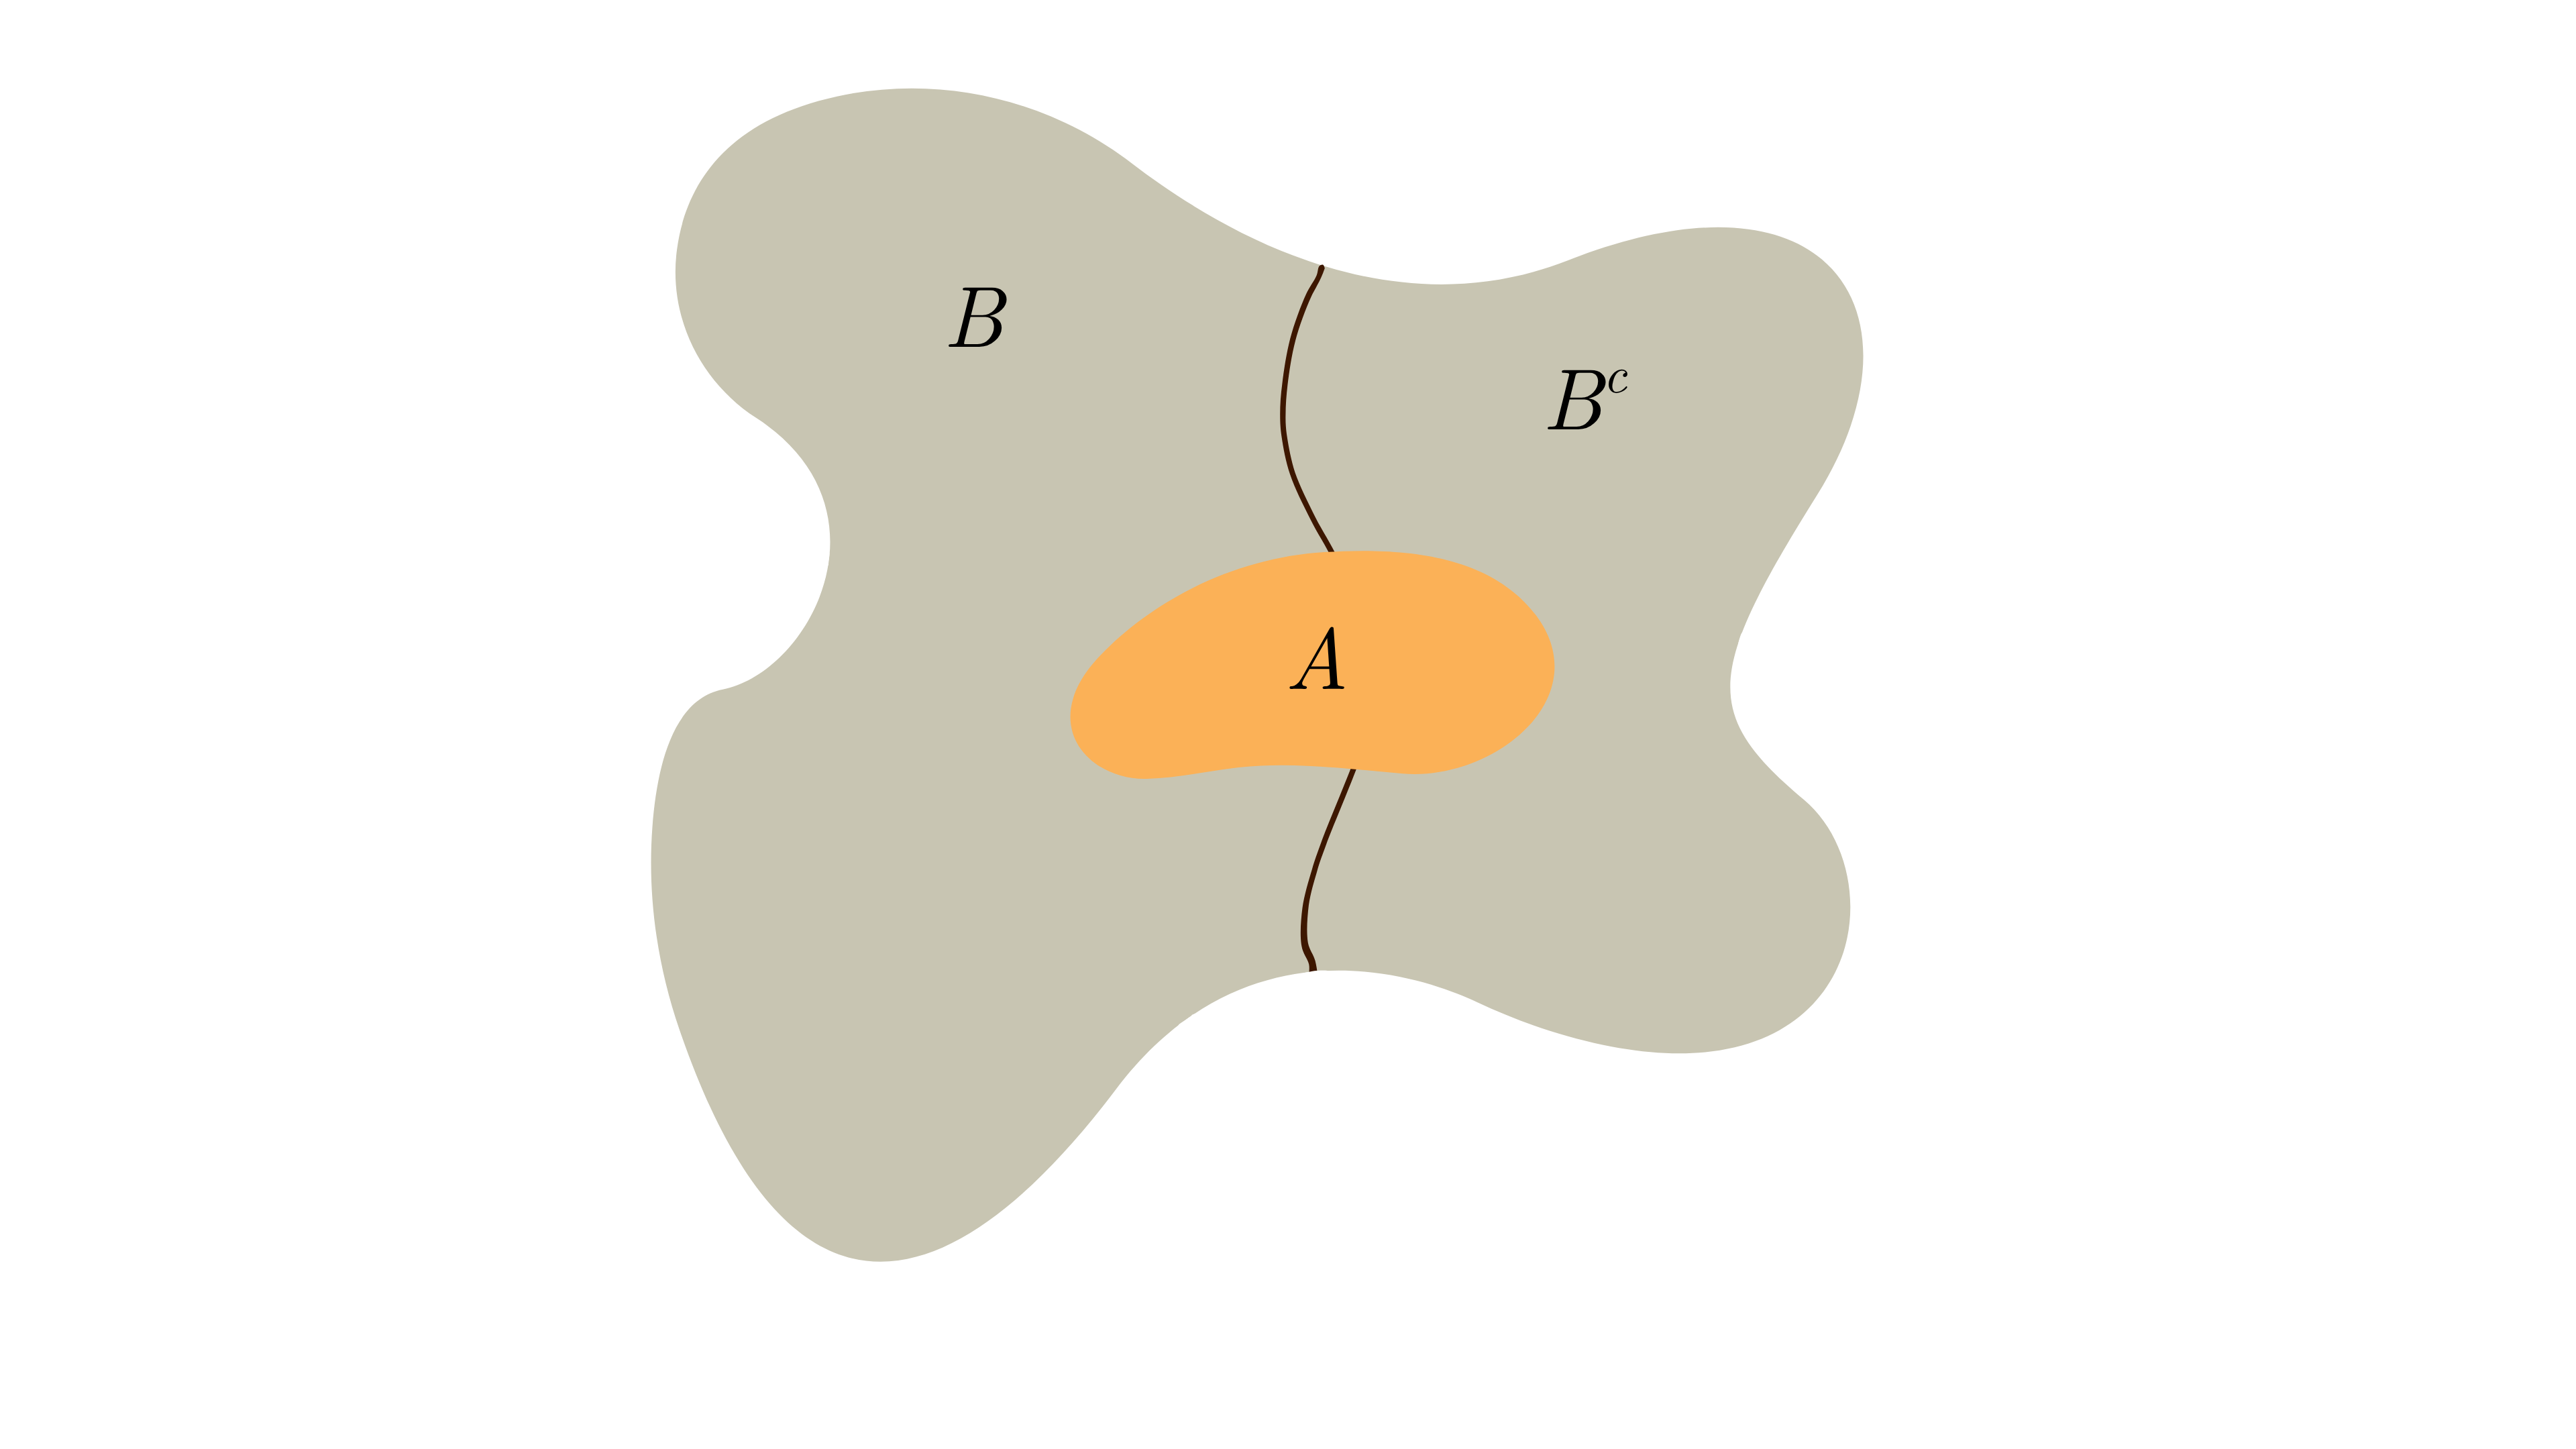
\includegraphics[trim={13cm 0 13cm 0},clip,width=0.5\linewidth]{chapters/chapter 8/total probability 1.png} }}%
    % \qquad
    \subfloat{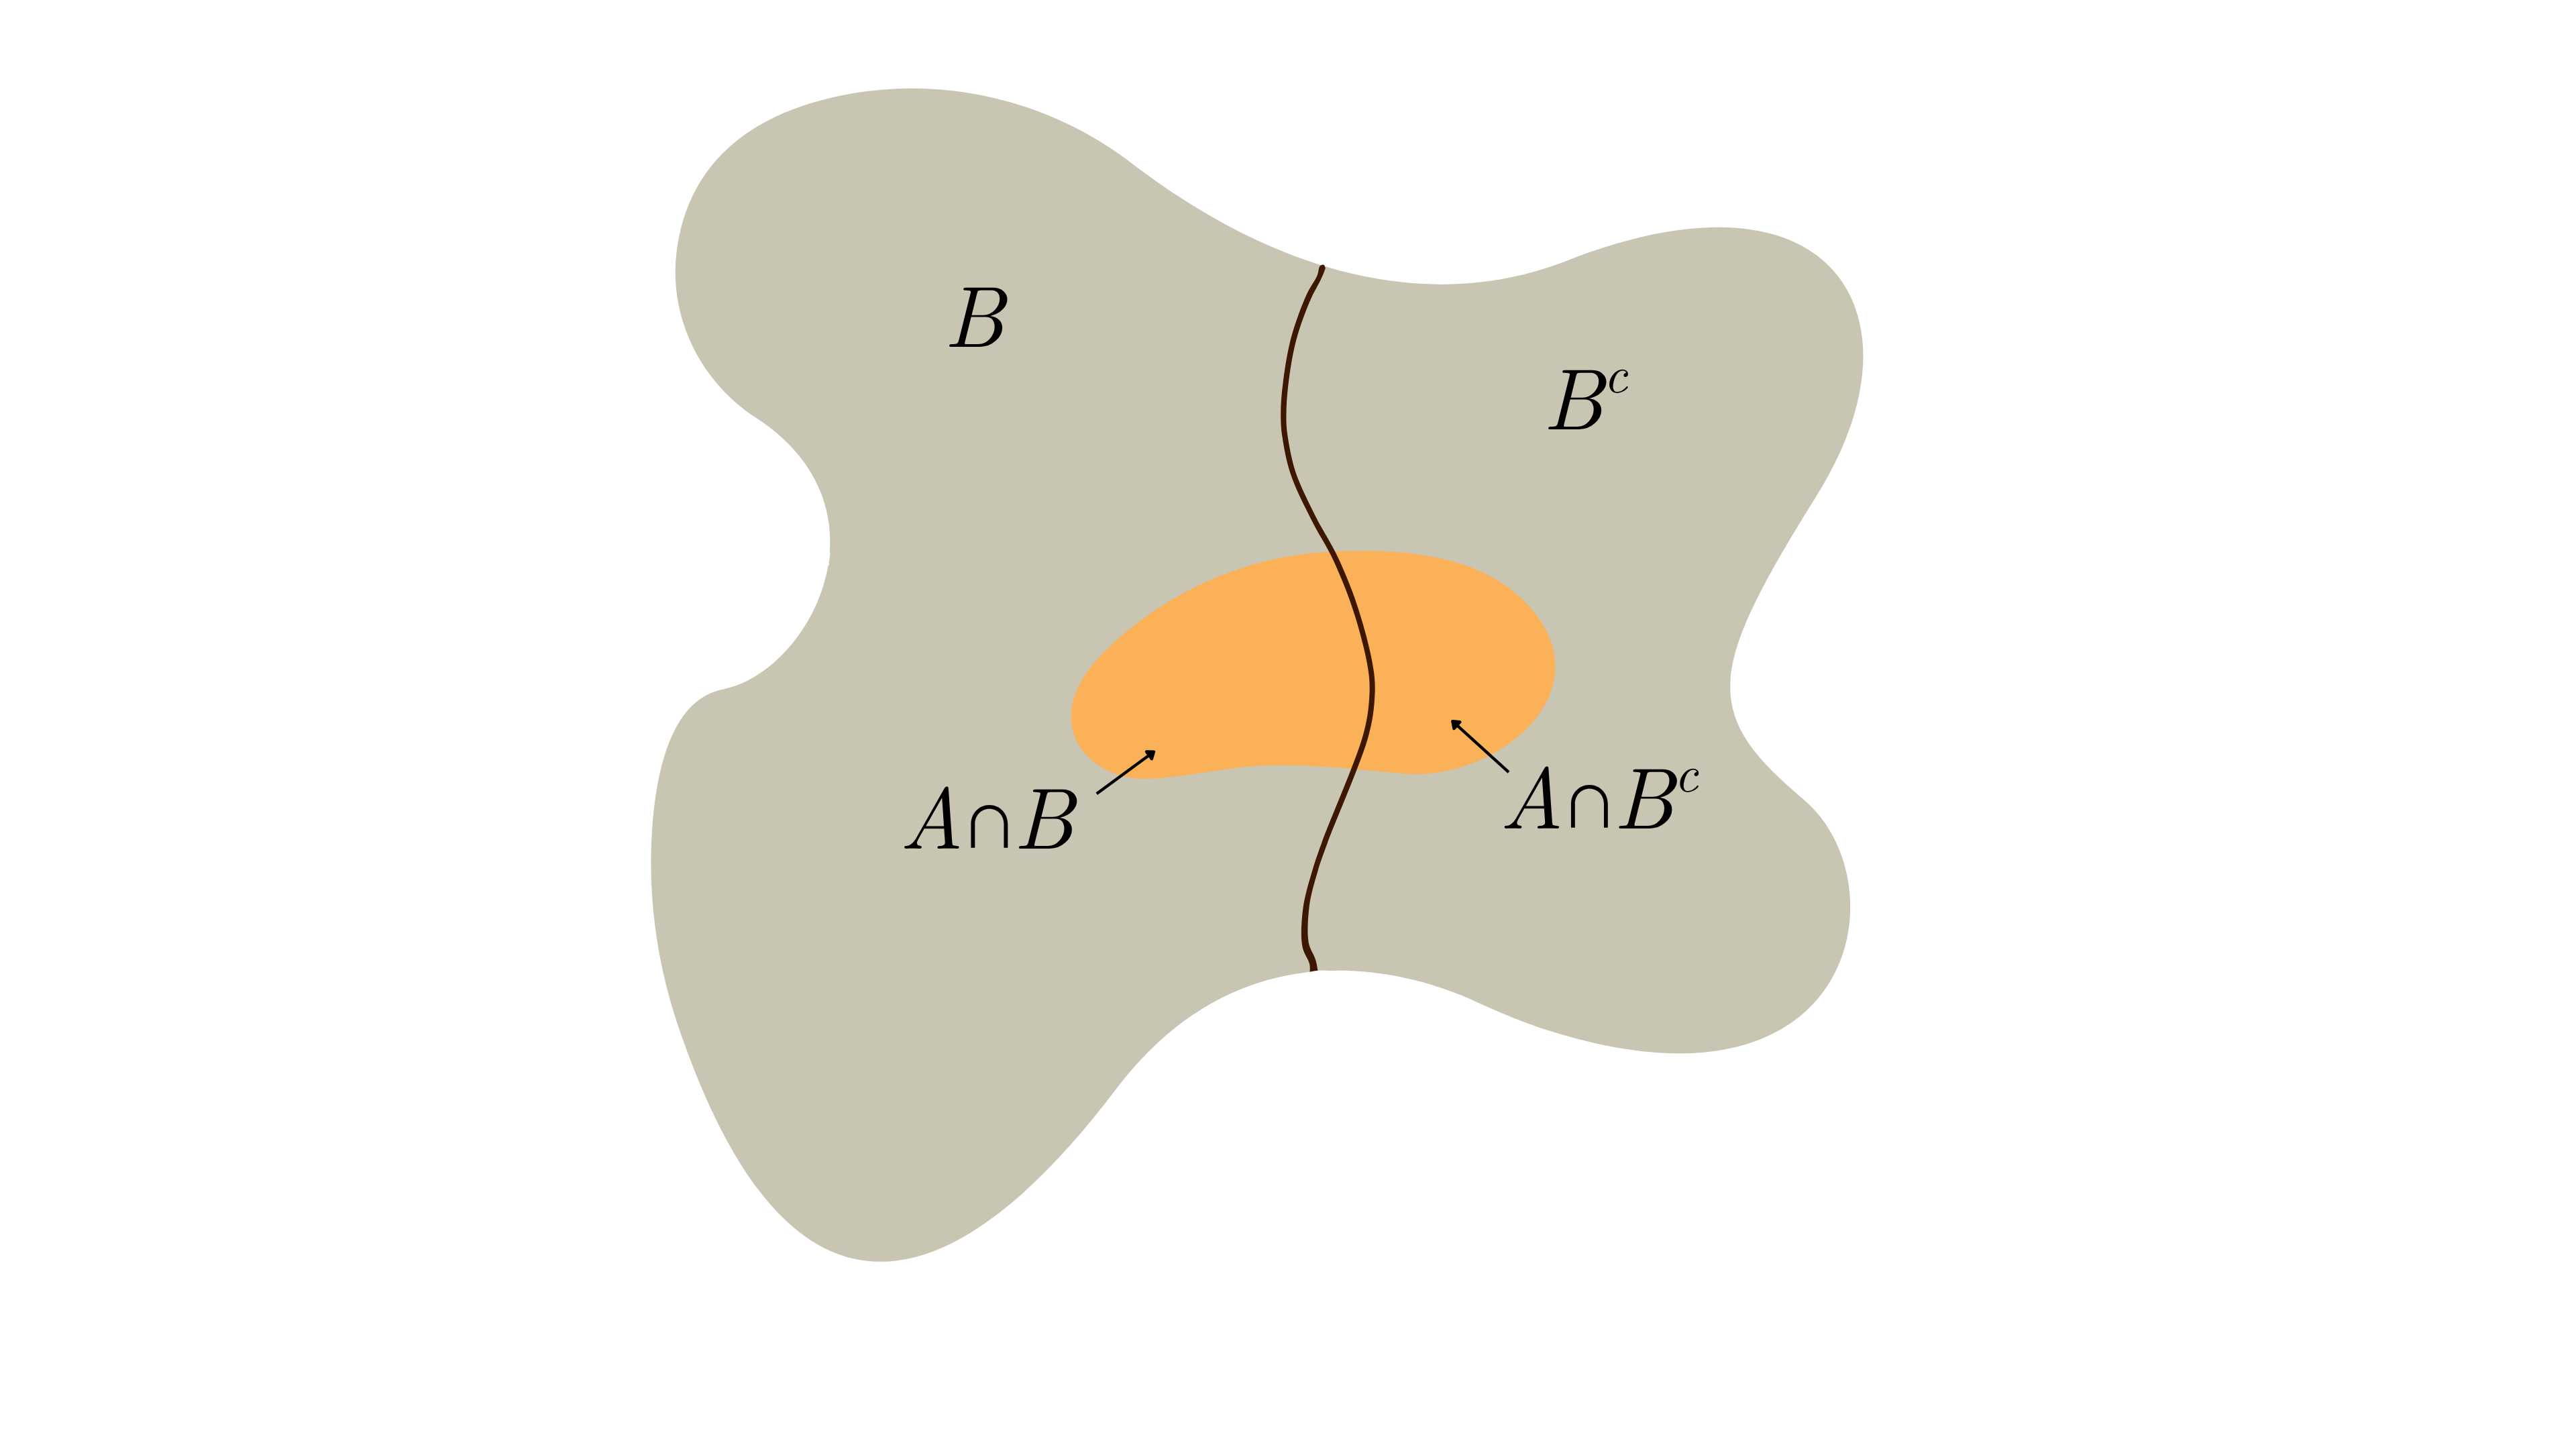
\includegraphics[trim={13cm 0 13cm 0},clip,width=0.5\linewidth]{chapters/chapter 8/total probability 2.png}} %
\end{figure}

Այստեղ արդեն օգտվելով պայմանական հավանականությունից՝
\begin{align*}
\PP[A] &= \PP[A \cap B] + \PP[A \cap B^c]
\\&= \PP[B] \cdot \PP[A \mid B] + \PP[B^c] \cdot \PP[A \mid B^c]
\\&= \frac{3}{5} \cdot 0.1 + \frac{2}{5} \cdot 0.15 = \frac{3}{25} = 0.12
\end{align*}
և խնդիրը լուծված է։ Ստացվածը կոչվում է \textit{լրիվ հավանականության բանաձև․}
\[
\PP[A] = \PP[B] \cdot \PP[A \mid B] + \PP[B^c] \cdot \PP[A \mid B^c]
\]
Ինչո՞ւ «լրիվ»։ Որովհետև կարծես բոլոր դեպքերը բաժանում ենք երկու ենթադեպքերի, յուրաքանչյուրում հաշվում, ապա համապատասխան կշիռներով\marginnote{ըստ էության՝ ենթադեպքերի գծային զուգակցությունն է} (դեպքերի հավանականություններով) բազմապատկելով ու գումարելով ստանում լրիվ հավանականությունը։

Անշուշտ, նույնը ճիշտ է նաև, եթե բաժանենք ոչ թե երկու, այլ երեք և ավելի չհատվող ենթադեպքերի․\begin{marginfigure}[*-2]
    \centering
    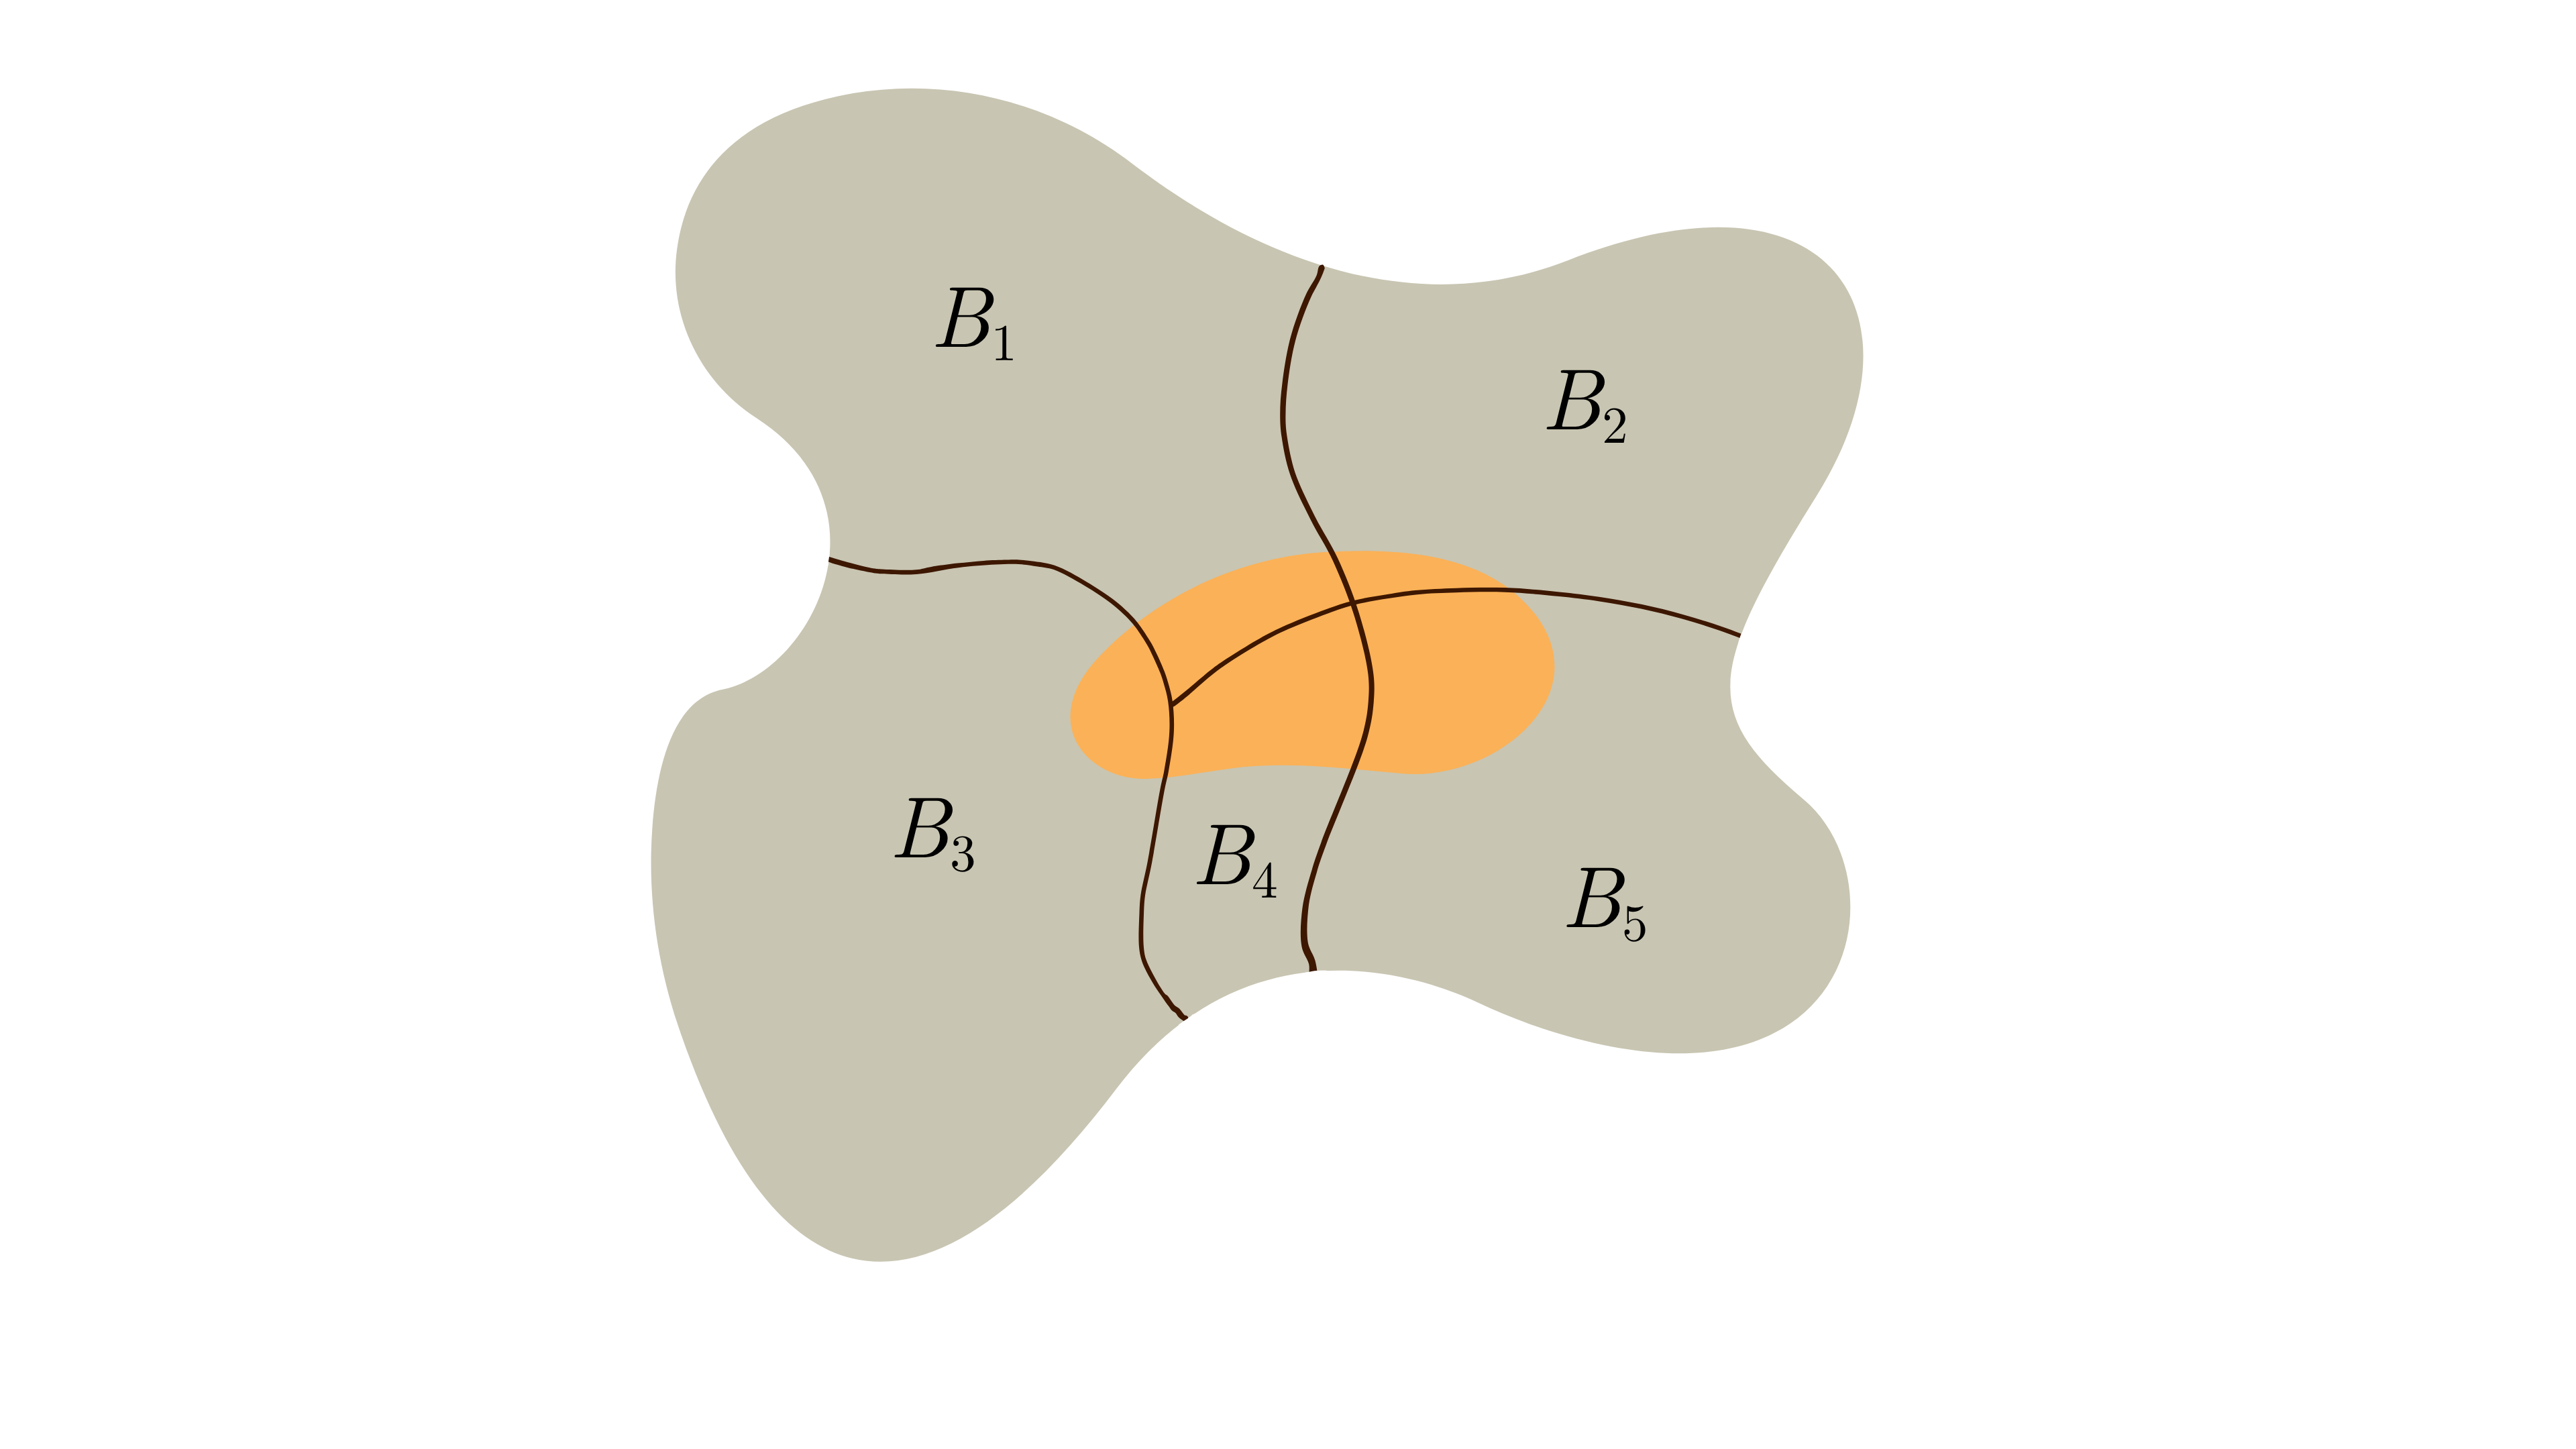
\includegraphics[trim={15cm 0 15cm 0},clip,width=\linewidth]{chapters/chapter 8/total probability generalized.png}
\end{marginfigure}
\begin{theorem}
Եթե $A$ պատահույթը կարելի է բաժանել մի քանի չհատվող պատահույթների միջև՝ $A \subset B_1 \cup B_2 \cup \dots$, ապա
\[
\PP[A] = \PP[B_1] \cdot \PP[A \mid B_1] + \PP[B_2] \cdot \PP[A \mid B_2] + \dots
\]
\end{theorem}

\warning{Բանաձևը ճիշտ է, միայն եթե $B_n$-երը \textbf{չեն հատվում։}}

\begin{example}
Ունենք $52$ խաղաթուղթ։ Պատահականորեն վերցնում ենք դրանցից մեկը, տակը մնում է $51$ հատ։ Որքա՞ն է հավանականու\-թյունը, որ եթե վերցնենք ևս մեկ խաղաթուղթ, այն կլինի սիրտ։\marginnote{սրտերը $13$ հատ են}

Նշանակենք՝
\begin{align*}
    A &= \text{երկրորդ հանածը սիրտ է} \\
    B &= \text{առաջին հանածը սիրտ է}
\end{align*}

\begin{marginfigure}
\resizebox{0.9\linewidth}{!}{%
\begin{tikzpicture}[scale=1]
% 1st level
\draw[very thick, blue]%
   (0,0) 
   -- node[above, sloped, align=center]
      {\textcolor{black}{$1$-ինը $\heartsuit$ է}\\$(1/4=25\%)$} 
   (\wideOne,\distOne);
\draw[very thick, blue] 
   (0,0) 
   -- node[below, sloped, align=center]
      {\textcolor{black}{$1$-ինը $\heartsuit$ չէ}\\($3/4=75\%$)} 
   (\wideOne,-\distOne);

% 2nd, 3rd and 4th Level
\draw[very thick, blue] 
   (\wideOne,\distOne)
   -- node[above, align=center, sloped]
      {\textcolor{black}{$2$-րդը $\heartsuit$ է}\\$(12/51=23.53\%)$}
   ++ (\wideTwo,\distTwo) 
   ; 
\draw[thick] 
   (\wideOne,\distOne) 
   -- node[below, align=center, sloped]
      {$2$-րդը $\heartsuit$ չէ}
   ++ (\wideTwo,-\distTwo) 
   ;
\draw[very thick, blue] 
   (\wideOne,-\distOne) 
   -- node[above, align=center, sloped]
      {\textcolor{black}{$2$-րդը $\heartsuit$ է}\\$(13/51=25.49\%)$}
   ++ (\wideTwo,\distTwo) 
   ;  
\draw[thick] 
   (\wideOne,-\distOne)
   -- node[below, align=center, sloped]
      {$2$-րդը $\heartsuit$ չէ}
   ++ (\wideTwo,-\distTwo) 
   ; 
\end{tikzpicture}
}
\end{marginfigure}
Առաջին խաղաթուղթը հանելուց հետո
\begin{itemize}
    \item եթե հանվածը սիրտ է, ապա մնում է ևս $12$ սիրտ
    \item եթե հանվածը սիրտ չէ, ապա մնում է $13$ սիրտ
\end{itemize}
այսինքն՝ $\PP[A \mid B] = \dfrac{12}{51}$ և $\PP[A \mid B^c] = \dfrac{13}{51}$:

Մյուս կողմից $\PP[B] = \dfrac{13}{52}$, հետևաբար լրիվ հավանականությունն է՝
\[ 
\PP[A] =
\PP[B]\cdot \PP[A\mid B] + \PP[B^c] \cdot \PP[A \mid B^c] =
\frac{13}{52}\cdot \frac{12}{51} + \frac{39}{52}\cdot \frac{13}{51} = \frac{1}{4}
\]
Կարո՞ղ էիք պատասխանը ստանալ այլ եղանակով։
\end{example}


\section{Անկախություն}

Վերևում հաշվեցինք զառը կամ մետաղադրամը նետելիս ստացվող տարբեր պատահույթների հավանականություններ։ Իսկ ի՞նչ, եթե կա\-տա\-րենք այսպիսի փորձ․ միաժամանակ նետենք զառը և մետաղադրամը։ Որևէ ազդեցություն կունենա՞ արդյոք զառի ընկած թիվը մետաղադրամի արդյունքի վրա։ Կփոխվի՞, ասենք, զառի $3$ ընկնելու հավանականու\-թյու\-նը, եթե իմանաք, որ մետաղադրամը գիր է ընկել։ Իհարկե ոչ․ զառը նույն\-իսկ տեղյակ չէ, որ Դուք իրենից բացի մետաղադրամ եք նետել, և դրան\-ցից մեկը մյուսի վրա ոչ մի ազդեցություն չունի։

Նույն կերպ իրարից կախում չունեն 
\begin{itemize}
    \item մետաղադրամների երկու տարբեր նետումները
    \item իրար հետևից կամ թեկուզ միաժամանակ նետված երկու զառերը
    \item միևնույն զառի առաջին և երկրորդ նետումները
    \item պատահական վերցված երկու մարդկանց հասակները
\end{itemize}
և այլն։ Այլ կերպ ասած՝ դրանք անկախ են։

\begin{definition}
Կասենք, որ $A$ և $B$ պատահույթներն \textbf{անկախ} են, եթե 
\[
\PP[A \cap B] = \PP[A] \cdot \PP[B]
\]
կամ համարժեքորեն՝\marginnote{երկու կողմը բաժանենք $\PP[B]$-ի}
\[
\PP[A \mid B] = \PP[A]
\]
\end{definition}

Երկրորդ պայմանը նշանակում է, որ $A$ պատահույթի համար $B$-ն եղած-չեղած մի հաշիվ է․ $A$-ի հավանականությունը $B$ պայմանի դեպքում նույնն է, ինչ առանց $B$ պայմանի։  

\begin{example}
Վերջին անգամ նետենք երկու զառ։ Նշանակենք՝
\begin{align*}
    A &= \text{առաջին զառը զույգ է} \\
    B &= \text{երկրորդ զառը կենտ է}
\end{align*}
Պարզենք, թե որքան է $A \cap B$ պատահույթի հավանականությունը։

Նախ $\PP[A] = \PP[B] = \dfrac{3}{6} = 0.5$։ Քանի որ զառերի ելքերն իրարից անկախ են, ապա հավանականությունը, որ միաժամանակ առաջին զառը կլինի զույգ, իսկ երկրորդը՝ կենտ, հավասար է
\[
\PP[A \cap B] = \PP[A] \cdot \PP[B] = \frac{1}{2} \cdot \frac{1}{2} = 0.25
\]
% առանց ավելորդ հաշվարկների։
\end{example}

\question{Նետում ենք $100$ զառ։ Որքա՞ն է հավանական, որ բոլորը կընկնեն զույգ։ Իսկ որ գոնե մեկը կընկնի կե՞նտ։}

\begin{example}
Մոտենում եք երկու պատահական անցորդի, հարցնում, թե նրանք որ ամսին են ծնվել, և եթե այն համընկնում է Ձեր ծնված ամսվա հետ, ապա ուրախանում եք։ Որքա՞ն է հավանական, որ երկու հոգուց գոնե մեկի ամիսը կհամընկնի Ձերինի հետ։

Եթե $A_1$-ով նշանակենք առաջին, իսկ $A_2$-ով՝ երկրորդ անցորդի ծննդյան ամսվա համընկնելը Ձեր ամսվա հետ, ապա
\begin{itemize}
    \item $A_1$-ն ու $A_2$-ը կլինեն անկախ
    \item ընդ որում $\PP[A_1] = \dfrac{1}{12}$ և $\PP[A_2] = \dfrac{1}{12}$ 
\end{itemize}

Մեր նպատակն է հաշվել $A_1$-ից ու $A_2$-ից գոնե մեկի տեղի ունենալու հավանականությունը, հետևաբար՝
\begin{align*}
\PP[A_1 \cup A_2] &= \PP[A_1] + \PP[A_2] - \PP[A_1 \cap A_2] \\&= \PP[A_1] + \PP[A_2] - \PP[A_1] \cdot \PP[A_2] \\&= \frac{1}{12} + \frac{1}{12} - \frac{1}{12^2} = \frac{23}{144} \approx 0.16
\end{align*}
\end{example}

Նկատենք նաև, որ եթե երկու $A$ ու $B$ պատահույթներ անկախ են, \marginnote{ասենք $1$-ին զառի զույգ լինելն ու $2$-րդի կենտ լինելը} ապա նրանց լրացումները`
\begin{itemize}
    \item $A^c$-ն ու $B$-ն
    \item $A^c$-ն ու $B^c$-ն
    \item $A$-ն ու $B^c$-ն
\end{itemize}
նույնպես անկախ են։ Այսինքն եթե $A$-ի տեղի ունենալը չի ազդում $B$-ի հավանականության վրա, ապա բնականաբար $A$-ի տեղի չունենալը նույնպես չի ազդում $B$-ի վրա։

Նման ձևով, եթե մի պատահույթի տեղի ունենալուց հետևում է, որ մյուսը չի կարող տեղի ունենալ (այսինքն դրանք չեն հատվում՝ անհամատեղելի են), ապա այդ երկուսի միջև ինչ-որ կապ կա, և դրանք անկախ չեն։ Հետևաբար,
\begin{theorem}
Եթե $A$ և $B$ պատահույթներն անկախ են\marginnote{և եթե $\PP[A]$, $\PP[B]$ $\ne 0$}, ապա նրանք չեն կարող անհամատեղելի լինել։
\end{theorem}

\question{Կարո՞ղ եք ապացուցել թեորեմը։}


\section{Երկրաչափական հավանականություն}

Հավանականային խնդիրները լուծելու ամենահաճելի ձևերից է դրանց երկրաչափորեն մոտենալը։

\question{$AD$ հատվածից պատահականորեն վերցնում ենք որևէ կետ։ Ի՞նչ եք կարծում, որքան է հավանական, որ այն կգտնվի $B$ և $C$ կետերի միջև։}
\begin{figure}[h]
\centering
\begin{tikzpicture}[scale=0.65]
  \draw[<->, myblue] (-6.5,0) -- (6.5,0);
  \foreach \x in {-6,...,6} {
    \draw (\x,0.1) -- (\x,-0.1);
    \pgfmathparse{mod(\x,3)==0}
      \ifnum\pgfmathresult=1
        \node[below] at (\x,-0.1) {$\x$};
      \fi
  }
  \node at (-5,0.5) {$A$};
  \node at (-2,0.5) {$B$};
  \node at (3,0.5) {$C$};
  \node at (6,0.5) {$D$};
\end{tikzpicture}
\end{figure}

Ի՞նչ նկատի ունենք «երկրաչափորեն» ասելով․ եթե բոլոր ելքերը հավասարահավանական են, ապա $\PP[A]$-ն հաշվելու համար
\begin{enumerate}
    \item բոլոր ելքերի $\Omega$ բազմությունը պատկերում ենք հատվածի, շրջանի, քառակուսու կամ այլ երկրաչափական պատկերի միջոցով
    \item նույնը անում ենք $A$-ի համար, այսինքն վերցնում ենք $\Omega$-ի այն մասը, որի կետերը բավարարում են մեր $A$ պատահույթին
    \item նշված մասի ($A$-ի) երկարությունը/մակերեսը բաժանում ենք ընդ\-հանուրի վրա
\end{enumerate}

\begin{example}
Ավտոբուսը գալիս է $12$:$00$-$13$:$00$ ընկած պատահական պահի։\marginnote{բոլոր պահերը նույն հավանականու\-թյամբ} Որքա՞ն է հավանականությունը, որ ավտոբուսը բաց չենք թողնի, եթե $12$:$30$-ին լինենք կանգառում։

\begin{center}
\begin{tikzpicture}
    \draw[-, thick] (-1.3,0) -- (7.3,0);
    
    \draw[thick, myred] (0,0) -- (3,0);
    \draw[thick, mygreen] (3,0) -- (6,0);
    
    \foreach \x in {0,3,6} {
    \draw[thick] (\x,0.15) -- (\x,-0.15);
    }
    
    \node[below, align=center] at (0,-0.15) {$0$};
    \node[below, align=center] at (3,-0.15) {$30$};
    \node[below, align=center] at (6,-0.15) {$60$};
    
    \node[myred, above, align=center] at (1.5,0.1) {\text{բաց կթողնենք}};
    \node[mygreen, above, align=center] at (4.5,0.1) {\text{կհասնենք}};
\end{tikzpicture}
\end{center}
Նախ նկարենք ավտոբուսի գալու ժամանակահատվածը՝ $12$:$00$-$13$:$00$, որը կլինի $60$ երկարությամբ հատված։ Ապա նրա վրա նշենք այն հատվածը, որում գալու դեպքում ավտոբուսը բաց չենք թողնի։ Կունենանք $[0, 30]$ հատվածը, որի երկարությունը բաժանելով ընդհանուրի վրա՝
\[
\PP[\text{կհասնենք}] = \frac{30}{60} = 0.5
\]
\end{example}

\begin{marginfigure}
\centering
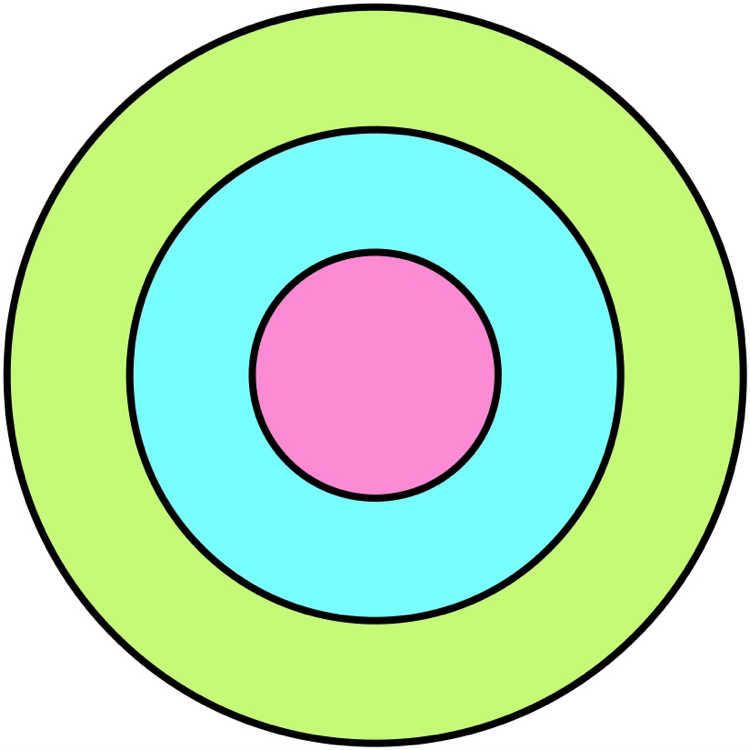
\includegraphics[width=0.75\linewidth]{chapters/chapter 8/concentric circles.png}
\caption*{$r$ շառավղով շրջանի մակերեսն է $\pi r^2$}
\end{marginfigure}

Դե իսկ եթե պատկերները ոչ թե հատվածներ են, այլ երկչափ պատ\-կեր\-ներ, երկարության փոխարեն կբաժանենք դրանց \href{http://qarakusi.am/lesson/119}{մակերեսները}։

\question{Շրջանների շառավիղներն են $1$, $2$ և $3$։ Որքա՞ն է հավա\-նա\-կան, որ պատահականորեն ընտրված կետը կգտնվի վարդագույն շրջանի մեջ։}

Երկրաչափորեն լուծենք մի փոքր ավելի հետաքրքիր խնդիր, որն առաջին հայացքից այնքան էլ երկրաչափական տեսք չունի։ 

Ենթադրենք հայտնի է, որ ավտոբուսը կանգառ է ժամանում $12$:$00$-$13$:$00$ ժամանակահատվածում ինչ-որ պատահական պահի, $5$ րոպե սպասում և շարժվում։ Մենք նույնպես կանգառ ենք գալիս $12$:$00$-$13$:$00$ ընկած որևէ պատահական պահի, սպասում մինչև $20$ րոպե, և եթե $20$ րոպեից ավտոբուսը չի գալիս, ոտքով հեռանում։ Փորձենք պարզել, թե որքա՞ն է հավանականությունը, որ ավտոբուս կնստենք։

Նախ որո՞նք են հնարավոր ելքերը։ Քանի որ ունենք երկու անհայտ մեծություններ, որոնք պատահական արժեքներ են ընդունում $12$:$00$-ից $13$:$00$-ի միջև, կամ որ նույնն է՝ $[0, 60]$ միջակայքում, ապա բոլոր ելքերը կարող ենք պատկերել $60 \times 60$ քառակուսու միջոցով՝
\begin{figure}[h]
\centering    
\caption*{սա մեր $\Omega$-ն է}
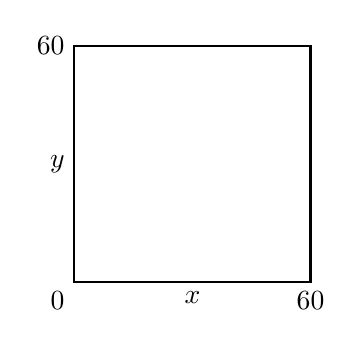
\begin{tikzpicture}[scale=0.05]  
  \draw[thick] (0,0) rectangle (60,60);
  
  \node[left] at (0,60) {$60$};
  \node[below] at (60,0) {$60$};
  \node[below] at (30,0) {$x$};
  \node[left] at (0,30) {$y$};
  \node[below left] at (0,0) {$0$};
\end{tikzpicture}    
\end{figure}

Հարմարության համար $x$-ով նշանակենք մեր գալու պահը, իսկ $y$-ով՝ ավտոբուսինը․ $(6, 34)$ կետը, օրինակ, ցույց կտա այն ելքը, երբ մենք կանգառ ենք հասել $12$:$06$ րոպեին, իսկ ավտոբուսը $12$:$34$-ին։ Իհարկե այդ իրավիճակում մենք դեռևս $12$:$26$ գնացած կլինենք և ավտոբուս չենք նստի։

Ո՞ր պատկերը ցույց կտա ավտոբուս նստելու պատահույթը։ Որպեսզի ավտոբուս նստենք, հարկավոր է, որ նախ մենք չուշանանք, այսինքն՝ գանք ավտոբուսի գնալուց ոչ ավել, քան $5$ րոպե հետո․
\[
y - x = \Big(\;\text{մեր գալու պահը}\;\Big) - \Big(\;\text{ավտոբուսի գալու պահը}\;\Big) \le 5
\]
կամ որ նույնն է՝ $y \le x + 5$։ Ուրեմն ավտոբուս նստելու համար $y$-ը պետք է գտնվի $y=x+5$ ուղղից ներքև։

\begin{figure}[t]
\centering

\begin{minipage}{0.48\textwidth}
\centering
\begin{tikzpicture}[scale=0.05]
  \fill[myLavender]
    (0,0) -- (0,5) -- (55,60) -- (60,60) -- (60,0) -- cycle;
  \draw[thick] (0,5) -- (55,60); 
  \draw[thick] (0,0) rectangle (60,60);
  \node[left] at (0,60) {$60$};
  \node[below] at (60,0) {$60$};
  \node[below] at (30,0) {$x$};
  \node[left] at (0,30) {$y$};
  \node[below left] at (0,0) {$0$};
  \node[rotate=45] at (27,40) {\small $y = x + 5$};
\end{tikzpicture}
\end{minipage}
\hfill
\begin{minipage}{0.48\textwidth}
\centering
\begin{tikzpicture}[scale=0.05]
  \fill[myOrange]
    (0,0) -- (0,60) -- (60,60) -- (60,40) -- (20,0) -- cycle;
  \draw[thick] (20,0) -- (60,40);
  \draw[thick] (0,0) rectangle (60,60);
  \node[left] at (0,60) {$60$};
  \node[below] at (60,0) {$60$};
  \node[below] at (30,0) {$x$};
  \node[left] at (0,30) {$y$};
  \node[below left] at (0,0) {$0$};
  \node[rotate=45] at (43,15) {\small $y = x - 20$};
\end{tikzpicture}
\end{minipage}

\end{figure}

Մյուս կողմից՝ եթե գանք ավտոբուսից $20$+ րոպե շուտ, ապա $20$ րոպեից կշարունակենք քայլել և նորից չենք նստի ավտոբուս։ Ուրեմն ավտոբուս նստելու համար հարկավոր է, որ
\[
x - y = \Big(\;\text{ավտոբուսի գալու պահը}\;\Big) - \Big(\;\text{մեր գալու պահը}\;\Big) \le 20
\]
կամ որ նույնն է՝ $y \ge x - 20$․ $y$-ը գտնվի $y=x-20$ ուղղից վերև։

Երկրաչափորեն այս տիրույթներից յուրաքանչյուրը մեր քառակուսու մեջ ընկած ինչ-որ հնգանկյուններ են, և այն կետերը, որոնք միաժամանակ երկուսում էլ գտնվում են, հենց այն ելքերն են, երբ ոչ մենք ենք ուշանում, ոչ ավտոբուսը։ Հետևաբար մեզ անհրաժեշտ ելքերի բազմությունը այս հնգանկյունների հատումն է՝

\begin{figure}[h]
\centering
\begin{tikzpicture}[scale=0.05]  
  \fill[mygreen, opacity=0.7]
    (0,0)     
    -- (0,5)  
    -- (55,60)
    -- (60,60)
    -- (60,40)
    -- (20,0) 
    -- cycle;
  \draw[thick] (0,5) -- (55,60); 
  \draw[thick] (20,0) -- (60,40);
  \draw[thick] (0,0) rectangle (60,60);
  \node[left] at (0,60) {$60$};
  \node[left] at (0,7.5) {$5$};
  \node[below] at (60,0) {$60$};
  % \node[below] at (30,0) {$x$};
  \node[below] at (20,0) {$20$};
  % \node[left] at (0,30) {$y$};
  \node[below left] at (0,0) {$0$};
\end{tikzpicture}
\caption*{սպիտակ եռանկյունների էջերը՝ $55$ և $40$}
\end{figure}

որի մակերեսը բաժանելով ամբողջ քառակուսու մակերեսին՝ կստանանք ավտոբուս նստելու հավանակա\-նու\-թյունը․
\[
\PP[\text{ավտոբուս նստել}] 
= 
\frac{\text{\color{mygreen} կանաչ մաս}}{\text{ընդհանուր}}
=
\frac{60^2-\frac{55^2}{2}-\frac{40^2}{2}}{60^2}
=
\frac{103}{288} \approx 0.36
\]


\bigskip 

\begin{theory}
.
\begin{itemize}
\item կարդալ [{\rm Grimmett-Welsh}], 3-5 էջերը (պատահույթներ)
\item կարդալ [{\rm Blitzstein-Hwang}], 8-13 (օրինակներ), 20-23 (հա\-վա\-նա\-կա\-նություն) էջերը 
\item ըստ ցանկության՝ [{\rm Grimmett-Welsh}], 6-10 էջերը
\item վերադառնալ [{\rm Blitzstein-Hwang}], 42-43, 49-52, 56-57 կամ [{\rm Grimmett-Welsh}], 11-15 էջերին
\item տեսնել հավանականության հաշվման տարբեր \href{https://dlsun.github.io/skis/foundations/classical-probability.html}{օրինակներ}
\item խաղալ \href{https://setosa.io/conditional}{պայմանական հավանականության} հետ 
\item դիտել {\rm 3b1b}-ի \href{https://www.youtu.be/HZGCoVF3YvM
}{տեսադասը} Բայեսի բանաձևի մասին
\item ըստ ցանկության՝ նաև մեկ այլ \href{https://youtu.be/R13BD8qKeTg}{տեսանյութ} 
\end{itemize}
\end{theory}

\newpage

\section{Խնդիրներ}

\begin{problem}
Նետում ենք երկու զառ։ Որքա՞ն է հավանականությունը, որ կընկնի
\begin{enumerate}[label={\alph*}․]
\item երկուսն էլ $3$
\item գոնե մեկ հատ $1$
\item ուղիղ մեկ հատ $1$
\item մեկ հատ $1$, մեկ հատ $4$
\item առաջինը՝ $1$, երկրորդը՝ $4$
\end{enumerate}
\end{problem}

\begin{problem}
Գրչատուփի մեջ կա $2$ սև, $5$ կապույտ և $6$ դեղին մատիտ։ Պատահականորեն վերցնում ենք դրանցից երկուսը։ Որքա՞ն է հավանա\-կան, որ երկու մատիտն էլ 
\begin{enumerate}[label={\alph*}․]
\item կարմիր կլինեն
\item նույն գույնի կլինեն
\item տարբեր գույների կլինեն
\item դեղին չեն լինի
\item կանաչ չեն լինի
\end{enumerate}
\end{problem}

\begin{problem}
\begin{marginfigure}
    \centering
    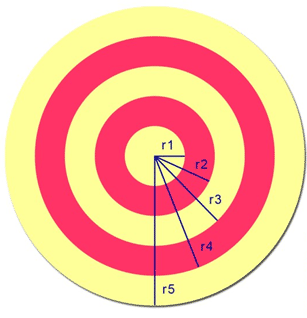
\includegraphics[width=\linewidth]{chapters/chapter 8/darts.png}
\end{marginfigure}
Նկարում պատկերված թիրախը կազմված է համապատաս\-խանաբար $1$, $2$, $3$, $4$ և $5$ սմ երկարությամբ շրջաններից։ Պատա\-հականորեն հարվածում ենք թիրախին։ Որքա՞ն է հավանականությունը, որ կդիպչենք
\begin{enumerate}[label={\alph*}․]
\item ամենափոքր շրջանին
\item կարմիր շրջանի
\item դեղին շրջանի
\end{enumerate}
\end{problem}

\begin{problem}
Մետաղադրամը նետում ենք $5$ անգամ։ Որքա՞ն է հավանակա\-նությունը, որ կենտ անգամ կընկնի գիր։
\end{problem}

\begin{problem}
Գրապահարանում կա $15$ գիրք, որոնցից $5$-ը հայերեն են, $10$-ը՝ ֆրանսերեն։ Ռուբենը ֆրանսերեն չգիտի։ Նա պատահականորեն վերցնում է $3$ գիրք։ Որքա՞ն է հավանականությունը, որ նա դրանցից գոնե մեկը կարող է կարդալ։
\end{problem}

\begin{problem}
Երեք անգամ նետում ենք զառը։ $A$, $B$, $C$-ով նշանակենք հետևյալ պատահույթները՝
\begin{itemize}
    \item $A$ $=$ գոնե մեկ անգամ ընկել է զույգ թիվ
    \item $B$ $=$ գոնե մեկ անգամ ընկել է $3$-ի պատիկ թիվ
    \item $C$ $=$ գոնե մեկ անգամ ընկել է $5$
\end{itemize}
Որքա՞ն է հավանականությունը, որ այս երեքից գոնե մեկը տեղի կունենա։
\end{problem}

\begin{problem}
Առաջին տուփում կա համապատասխանաբար $\{5, 11, 8\}$ սև, դեղին, կարմիր մատիտ, իսկ երկրորդում՝ $\{10, 8, 6\}$։ Յուրաքանչյուր տուփից պատահականորեն վերցնում ենք մեկական մատիտ։ Որքա՞ն է հավանականությունը, որ երկուսն էլ կլինեն նույն գույնի։
\end{problem}

\begin{problem}
Նետում ենք երկու զառ։ Որքա՞ն է հավանական, որ դրանցից մեկը կընկնի $1$, եթե գիտենք, որ դրանց գումարը զույգ է։
\end{problem}

\begin{problem}
$52$ խաղաթղթերից\marginnote[*+1.8]{հայերեն՝ քյափ}  պատահական վերցնում ենք $3$-ը։ Որքա՞ն է հավանականությունը, որ առաջին երկուսը կլինեն թագուհի (դամա), իսկ երրորդը՝ {\color{myred}$\blacklozenge$} աղյուս։
\end{problem}

\begin{problem}
Ցանկանում ենք գրել սպամերը հայտնաբերող ծրագիր։
Հայտնի է, որ
\begin{itemize}
    \item սպամ նամակների $80\%$-ը պարունակում է «շահեք» բառը
    \item ոչ սպամ նամակների $30\%$-ն է պարունակում «շահեք» բառը
    \item միջինում նամակների $40\%$-ը սպամ է
\end{itemize}
Ճիշտ այդ պահին ստանում ենք նամակ, որը պարունակում է «շահեք» բառը։ Որքա՞ն է հավանական, որ այն սպամ է։
\end{problem}

\begin{problem}
Երեք նորածինների տանում են ստուգելու, այնուհետև պատահականորեն վերադարձնում իրենց մայրերին։ Որքա՞ն է հավանա\-կանությունը, որ փոքրիկներից գոնե մեկին կվերադարձնեն իր մայրիկին։
\end{problem}

% \begin{problem}
% Suppose that you know the answers to 20 questions out of the total 25
% questions in the entrance examination, from which you are only asked
% 3 random questions. What is the probability that you answer all of
% the questions?

% \begin{problem}
% There are two boxes containing {5, 11} and {10, 8} white, black balls
% respectively. First, we take out a ball from each of the boxes. Then, we randomly choose one of them. What is the probability that the
% final ball is white?

% \begin{problem}
% There are three boxes having 4 white and 6 black balls in each of them.
% Suppose we perform the following steps in the given order:
%     \begin{enumerate}
%         \item[a) ] take out a ball from the first box and put it into the second one,
%         \item[b) ] take out a ball from the second box and put it into the third one,
%         \item[c) ] take out a ball from the third box and put it into the first one.
%     \end{enumerate}
%     What is the probability of taking a white ball from the third box (after doing \textit{a)-c)})?

\begin{problem}
Առաջին գործարանը երկրորդից $2$ անգամ ավելի շատ զենքեր է արտադրում։ Հայտնի է, որ 
\begin{itemize}
    \item առաջինում արտադրված զենքերի $40\%$-ը խոտան է
    \item երկրորդում արտադրվածների $16\%$-ն է խոտան
\end{itemize}
Պատահականորեն ստուգում ենք զենքերից մեկն ու պարզում, որ այն խոտանված չէ։ Որքա՞ն է հավանականությունը, որ այն արտադրել են առաջին գործարանում։
\end{problem}

\begin{problem}
Արձակուրդի գնալիս հարևանին խնդրում եք ամեն օր ջրել Ձեր ծաղիկները։ Եթե ծաղիկներն ամեն օր ջրեն, ապա $0.85$ հա\-վա\-նականությամբ դրանք կշարունակեն ծաղկել, մինչդեռ եթե չջրեն, ապա գոյատևելու հավանականությունն ընդամենը $0.2$ է։ Գրեթե $90\%$-ով համոզված եք, որ Ձեր հարևանը կջրի ծաղիկները, սակայն արձակուրդից վերադառնալով՝ տեսնում եք, որ ծաղիկները թառամել են։ 

Որքա՞ն է հավանական, որ հարևանը մոռացել է ջրել ծաղիկները։ Կշարունակե՞ք վստահել նրան։
\end{problem}

\begin{problem}
Նունեն դեպքերի $30\%$ տոկոսում մեքենայով է գործի գալիս, $30\%$-ում՝ ոտքով, իսկ մնացած $40\%$-ում գալիս է ավտոբուսով։ Ընդ որում,
\begin{itemize}
    \item ոտքով գալիս ուշանում է դեպքերի $10\%$-ում
    \item մեքենայով գալիս՝ $3\%$-ում
    \item ավտոբուսով գալիս՝ $7\%$-ում
\end{itemize}
Երեկ Նունեն ուշացել է։ Որքա՞ն է հավանականությունը, որ նա ավտո\-բու\-սով էր գալիս։ Որքա՞ն է հավանական, որ այսօր նա ոտքով էր, եթե այսօր ճիշտ ժամանակին է եկել։
\end{problem}

\begin{problem}
Անգետիկն ունի $10$ մետաղադրամ, որոնցից $9$-ը սովորական են, իսկ $1$-ի երկու կողմն էլ գիր է։ Նա պատահականորեն վերցնում է մետաղադրամներից մեկը․
\begin{enumerate}[label={\alph*}․]
\item որքա՞ն է հավանականությունը, որ դա կեղծ մետաղադրամն է

\item եթե նա նետի մետաղադրամն, ու այն գիր ընկնի, որքա՞ն է հավանականությունը, որ դա կեղծն է

\item եթե նա նետի մետաղադրամն, ու այն ղուշ ընկնի, որքա՞ն է հավանականությունը, որ դա $9$ սովորականներից մեկն է
\end{enumerate}
\end{problem}

\begin{problem}
Գառնի-Գեղարդից վերադառնալով՝ Ձեր տեսախցիկը տանում եք արհեստանոց՝ լուսանկարները մշակելու։ Ցավոք, արհես\-տա\-նոցում ժապավենը փչացնում են, և ընդհանուր $24$ կադրերից $4$ հաջոր\-դական կադրեր վնասվում են։ Որքա՞ն է հավանականությունը, որ վնասված կադրերի թվում են
\begin{enumerate}[label={\alph*}․]
\item ութերորդ, իններորդ կամ տասներորդ լուսանկարները
\item ութերորդ, իններորդ և տասներորդ լուսանկարները
\end{enumerate}
\end{problem}

\begin{problem}\marginnote[*+0.5]{\href{https://youtu.be/U2AE4TZU4MA}{լուծում}}
Անուշն ու Նաիրին ժամը $12$:$00$-ից $13$:$00$ որևէ պատահական պահի գալիս են «Մոսկվա» կինոթատրոնի մոտ և սպասում մյուսին՝ միասին ընդմիջման գնալու համար։ Եթե երկրորդը $15$ րոպեից ավել է ուշանում, առաջինը տեղ հասնողը միայնակ է գնում ընդմիջման։ 

Որքա՞ն է հավանականությունը, որ նրանք միասին կընդմիջեն, եթե երկուսի համար էլ $12$:$00$-$13$:$00$ բոլոր պահերը հավասարահավանական են։
\end{problem}

